%% Template para dissertacao/tese na classe UFBAthesis
%% versao 1.0
%% (c) 2005 Paulo G. S. Fonseca
%% (c) 2012 Antonio Terceiro
%% (c) 2014 Christina von Flach
%% www.dcc.ufba.br/~flach/ufbathesis

%% Carrega a classe ufbathesis
%% Opcoes: * Idiomas
%%           pt   - portugues (padrao)
%%           en   - ingles
%%         * Tipo do Texto
%%           bsc  - para monografias de graduacao
%%           msc  - para dissertacoes de mestrado (padrao)
%%           qual - exame de qualificacao de mestrado
%%           prop - exame de qualificacao de doutorado
%%           phd  - para teses de doutorado
%%         * Media
%%           scr  - para versao eletronica (PDF) / consulte o guia do usuario
%%         * Estilo
%%           classic - estilo original a la TAOCP (deprecated) - apesar de deprecated, manter esse.
%%           std     - novo estilo a la CUP (padrao)
%%         * Paginacao
%%           oneside - para impressao em face unica
%%           twoside - para impressao em frente e verso (padrao)

% Atenção: Manter 'classic' na declaracao abaixo:
\documentclass[qual, classic, a4paper]{ufbathesis}

%% Preambulo:
\usepackage[utf8]{inputenc}

%\usepackage[authoryear]{natbib}
\usepackage{graphicx}
\usepackage{lipsum}
\usepackage{hyphenat}
\usepackage[usenames, dvipsnames, table]{xcolor}
\usepackage{booktabs}
\usepackage{pifont}
\usepackage{multirow}
\usepackage{listings} 
\usepackage{colortbl}
\usepackage{xfrac}
\usepackage[FIGTOPCAP]{subfigure}
\usepackage{tabularx}
\usepackage{ragged2e}
\usepackage{acronym}
\usepackage{float}
\usepackage{todonotes}
\usepackage{amssymb}
\usepackage{placeins}
\usepackage{arydshln}

\presetkeys%
    {todonotes}%
    {inline,backgroundcolor=yellow}{}
    
\usepackage{blindtext}

\usepackage{tikz}
\usetikzlibrary{arrows,shapes,positioning,shadows,trees}

% Siglas
\acrodef{AM}[AM]{{Aprendizado de Máquina}}
\acrodef{DE}[DE] {{Distância Euclidiana}}
\acrodef{FCD}[FCD] {{\textit {Fluxo de Dados Contínuos}}}
\acrodef{DN}[DN] {{\textit {Detecção de Novidade}}}

% Universidade
\university{Universidade Federal da Bahia}

% Endereco (cidade)
\address{Salvador}

% Instituto ou Centro Academico
\institute{Instituto de Matem\'{a}tica}

% Nome da biblioteca - usado na ficha catalografica
\library{Biblioteca Reitor Mac\^{e}do Costa}

% Programa de pos-graduacao
\program{Programa de P\'{o}s-Gradua\c{c}\~{a}o em Ci\^{e}ncia da Computa\c{c}\~{a}o}

% Area de titulacao
\majorfield{Ci\^{e}ncia da Computa\c{c}\~{a}o}

% Titulo da dissertacao
\title{Aplicando redes de função de base radial para detecção de mudanças de conceito em fluxos contínuos de dados}

% Data da defesa
% e.g. \date{19 de fevereiro de 2013}
\date{03 de Abril de 2019}
% e.g. \defenseyear{2013}
\defenseyear{2019}

% Autor
% e.g. \author{Jose da Silva}
\author{Ruivaldo Azevedo Lobão Neto}

% Orientador(a)
% Opcao: [f] - para orientador do sexo feminino
% e.g. \adviser[f]{Profa. Dra. Maria Santos}
\adviser{Ricardo Ara\'{u}jo Rios}

% Orientador(a)
% Opcao: [f] - para orientador do sexo feminino
% e.g. \coadviser{Prof. Dr. Pedro Pedreira}
% Comente se nao ha co-orientador
%\coadviser{Nome Completo do CO-ORIENTADOR}

%% Inicio do documento
\begin{document}

\pgcompfrontpage

%% Parte pre-textual
\frontmatter

\pgcomppresentationpage

%%%%%%%%%%%%%%%%%%%%%%%%%
% Ficha catalografica
%%%%%%%%%%%%%%%%%%%%%%%%%

%\authorcitationname{Silva, Mirlei Moura da } % e.g. Terceiro, Antonio Soares de Azevedo
%\advisercitationname{Sobrenome, Nome do ORIENTADOR} % e.g. Chavez, Christina von Flach Garcia
%\coadvisercitationname{Sobrenome, Nome do CO-ORIENTADOR} % e.g. Mendonca, Manoel Gomes de
%\catalogtype{Disserta\c{c}\~{a}o (Mestrado)} % e.g. ou ``Tese (Doutorado)''

%\catalogtopics{1. Primeira palavra-chave. 2. Segunda palavra-chave. 3. Terceira palavra-chave} % Listar palavras-chave do trabalho para a FICHA CATALOGRAFICA}, por exemplo, ``1. Complexidade Estrutural. 2. Qualidade de Software 3. Engenharia de Software''
%\catalogcdd{XXX.XX} % e.g.  XXX.XX (número nesse formato serah dado pela biblioteca)
%\catalogcdu{XXX.XX.XXX} % e.g.  XXX.XX.XXX (idem) 
%\catalogingsheet

%%%%%%%%%%%%%%%%%%%%%
% Termo de aprovacaoo
%%%%%%%%%%%%%%%%%%%%%

\approvalsheet{Salvador, 03 de Abril de 2019}{
   \comittemember{Prof. Dr. Ricardo Araújo Rios}{UFBA}  
   %\comittemember{Profa. Dr...}{UFBA}
   %\comittemember{Prof. Dr...}{USP} 
}
   % Para mestrado, apenas 3.
   % \comittemember{Prof. Dr. Professor 4}{Universidade HJKL}
   % \comittemember{Profa. Dra. Professora 5}{Universidade QWERTY}

%%%%%%%%%%%%%%%%%%%%%%%%%%%%%%%%%%%%%%%% 
% Dedicatoria, Agradecimentos, Epigrafe
%%%%%%%%%%%%%%%%%%%%%%%%%%%%%%%%%%%%%%%%

% Comente para ocultar
%\begin{dedicatory}
%DIGITE A DEDICATORIA AQUI
%\end{dedicatory}

% Agradecimentos
% Se preferir, crie um arquivo `a parte e o inclua via \include{}
%\acknowledgements
%DIGITE OS AGRADECIMENTOS AQUI

% Epigrafe
%\begin{epigraph}[NOTA]{AUTOR}
%DIGITE AQUI A CITACAO
%\end{epigraph}

%%%%%%%%%%%%%%%%%%%%%
% Resumo 
%%%%%%%%%%%%%%%%%%%%%
\resumo

\blindtext

% Palavras-chave do resumo em Portugues
\begin{keywords}
    Aprendizado de Máquina, Fluxos Contínuos de Dados, Mudanças de Conceito, Redes de Função de Base Radial, Não supervisionado
\end{keywords}

\abstract

\blindtext

% Palavras-chave do resumo em Ingles
\begin{keywords}
    Machine Learning, Data Streams, Concept Drift, Radial Basis Function Networks, RBF Network, Unlabeled
\end{keywords}

%%%%%%%%%%%%%%%%%%%
% Sumario / Indice
%%%%%%%%%%%%%%%%%%%

% Comente para ocultar
\tableofcontents

% Lista de figuras
% Comente para ocultar
\listoffigures

% Lista de tabelas
% Comente para ocultar
\listoftables

%% Parte textual
\mainmatter

% Eh aconselhavel criar cada capitulo em um arquivo separado, digamos
% "capitulo1.tex", "capitulo2.tex", ... "capituloN.tex" e depois
% inclui-los com:
% \include{capitulo1}
% \include{capitulo2}
% ...
% \include{capituloN}
%
% Importante: 
% Use \xchapter{}{} ao inves de \chapter{}; se não quiser colocar texto antes do inicio do capitulo, use \xchapter{texto}{}.

%%%
\xchapter{Introdução}{} \label{introducao}

\section{Contexto e Motivação}

O volume de dados produzido por sistemas computacionais tem crescido de forma significativa nos últimos anos \cite{Cohen:BigData:2009:MSN:1687553.1687576}.
Em relatório publicado pelo IDC (\textit{International Data Corporation}), 
estimava-se que em 2014 seriam produzidos 4,4 zettabytes (trilhões de gigabytes) de dados 
e que em 2020 essa quantidade chegará a 44 zettabytes \cite{idc_report}.

Parte relevante desses dados é produzida em sequências contínuas, ordenadas, de alta frequência e potencialmente infinitas.
Estas sequências são denominadas Fluxos Contínuos de Dados (FCDs) e estão presentes em muitos domínios de aplicação, por exemplo \cite{Aggarwal:2006:DSM:1196418}: 
monitoramento de sensores \cite{Lee:Wang:Ryu:2007},
tráfico TCP/IP, 
histórico de compra de clientes,
filtragem de SPAM em mensagens de e-mail \cite{Katakis:2010:TRC:1746286.1746291},
detecção de intrusos,
análise de sentimentos \cite{Smailovic:2014:SAL:2941772.2941857}, 
etc.

A área de Aprendizado de Máquina (AM) estuda algoritmos que melhoram o seu desempenho na realização de determinada tarefa conforme ganham experiência \cite{Mitchell:1997:ML:541177}.
Nos últimos anos, há um crescente interesse de pesquisa no uso dessas técnicas em diferentes domínios de aplicação.
Em muitos desses domínios, os dados são produzidos através de fluxos contínuos de dados \cite{Aggarwal:2006:DSM:1196418}, sendo necessário, portanto, 
 adaptar os algoritmos para atenderem às restrições de tempo de execução e de uso dos recursos computacionais \cite{Bifet:2009:ALM:1656274.1656287}.

Além dessas restrições, a dinamicidade dos cenários com fluxos contínuos de dados também é considerada um obstáculo para as técnicas de aprendizado de máquina.
Isto ocorre, pois, nesses cenários, o contexto do processo ou a distribuição dos dados podem mudar ao longo do tempo, afetando as predições esperadas (conceitos-alvo).
Este problema é denominado mudança de conceito \cite{Gama:2010:KDD:1855075} e a sua ocorrência pode impactar a acurácia do modelo.

Visando mitigar esse problema, foram desenvolvidas técnicas para detecção de mudanças de conceito \cite{Gama:2014:SCD:2597757.2523813}.
As primeiras técnicas desenvolvidas atuavam em conjunto com os classificadores,  
detectando mudanças a partir do monitoramento da taxa de erro.
São exemplos desta abordagem: DDM \cite{GamaMCR04}, EDDM \cite{EDDM},  
ADWIN \cite{BifetG07}, ECDD \cite{Ross:2012:EWM:2076039.2076307}, 
PL \cite{Bach:PL:2008}, FCWM \cite{FCWM}, STEPD \cite{STEPD}, DOF \cite{Sobhani:2011:NDD:2045295.2045309}, 
SCCDD/CRCDD \cite{daCosta:2016:UDS:2956219.2956389}, dentre outros.

Os comitês de classificadores também foram utilizados em métodos para detecção de mudanças de conceito.
Nestes grupos, a predição global é obtida a partir da combinação das predições individuais.
Divergências identificadas durante este processo sinalizam potenciais mudanças de conceito \cite{Gama:2014:SCD:2597757.2523813}.
São exemplos desta técnica:
DWM \cite{Kolter:2007:DWM:1314498.1390333}, AUE \cite{AUE}, 
WMA \cite{Blum1997}, DDD \cite{Minku:2012:DNE:2197077.2197204}, ADOB \cite{deCarvalhoSantos:2014:SUR:3120352.3120365}, dentre outros.

Contudo, as abordagens mencionadas dependem que o rótulo correto de cada exemplo esteja disponível.
Em muitos contextos, o tempo ou o custo para obter esse rótulo é proibitivo \cite{Aggarwal:2006:DSM:1196418}.
Diante disso, foram desenvolvidos algoritmos que independem dessa informação.

As técnicas independentes de rótulos reconhecem as mudanças de conceito a partir da identificação de eventos que não se enquadram na estrutura dos dados conhecidos \cite{Spinosa:2007:OCA:1244002.1244107}.
Para tanto, técnicas de de agrupamento, detecção de \textit{outliers}, sumarização dos dados e aplicação de medidas de dissimilaridade são utilizadas nas implementações \cite{Ryu:Kantardzic:2012}.
São exemplos desta categoria:
OLINDDA \cite{Spinosa:2007:OCA:1244002.1244107},
MINAS \cite{Faria:2013:NDA:2480362.2480515},
ECSMiner \cite{Masud:2011:CNC:1978259.1978529},
GC3 \cite{Sethi2016b:GC3}, dentre outros.

Contudo, segundo \cite{Aggarwal:2006:DSM:1196418}, as técnicas para identificação de mudanças de conceito propostas ainda possuem deficiências.
Os algoritmos depentes de rótulos, por exemplo, são impraticáveis para muitos problemas do mundo real \cite{Gama:2014:SCD:2597757.2523813}.
De forma similar, as técnicas independentes têm dificuldade para atender às restrições de tempo de execução e de uso dos recursos computacionais em cenários com fluxos contínuos de dados.

Visando resolver essas limitações, este projeto de mestrado propõe um algoritmo baseado em redes de função de base radial capaz de detectar mudanças de conceito de forma online, precisa e idependente de exemplos prévios ou rótulos.

\section{Hipótese e Objetivo}

Com base nas observações citadas anteriormente, a seguinte hipótese foi formulada:

\begin{center}
\textit{``A análise de fluxos contínuos de dados através de redes de função de base radial permite a detecção de mudanças de conceito de forma online, precisa e idependente de exemplos prévios ou rótulos.''}
\end{center}

O objetivo deste trabalho será o desenvolvimento e comprovação desta hipótese.
Para atingir este objetivo, será implementado um algoritmo para detecção de mudanças de conceito baseado em redes de função de base radial. 
Os principais diferencias deste método serão a escolha dinâmica dos centros, conforme novos dados são recepcionados, e a aplicação de um raio variável.
A ativação de novos centros será utilizada como indicador de possíveis mudanças de conceito.

O algoritmo implementado será comparado com o estado da arte. 
O primeiro conjunto de testes será formado por dados sintéticos, que permitirão uma análise detalhada da abordagem, uma vez que as características e os comportamentos dos dados são conhecidos. 
O segundo conjunto será composto por dados obtidos a partir de sistemas computacionais utilizados na indústria,
visando apresentar uma aplicação prática para a solução proposta. 

Este projeto está organizado conforme a seguinte estrutura: 
O \textbf{Capítulo \ref{revisao_bibliografica}} apresenta uma revisão bibliográfica dos principais conceitos utilizados neste trabalho: fluxos contínuos de dados e aprendizado de máquina, mudança de conceito e redes de função de base radial; 
No \textbf{Capítulo \ref{plano_pesquisa}} o plano de pesquisa é detalhado, 
identificando a metodologia que será aplicada na pesquisa e o cronograma de atividades. 
Por fim, o \textbf{Capítulo \ref{experimentos_iniciais}} 
apresenta um conjunto de experimentos preliminares e a análise dos resultados obtidos.

\xchapter{Revisão Bibliográfica}{} \label{revisao_bibliografica}
\section{Considerações Iniciais}

Este capítulo discute os principais conceitos utilizados neste trabalho de pesquisa.
Em primeiro momento, a aplicação de técnicas de aprendizado de máquina a fluxos contínuos de dados será detalhada.
Em seguida, será apresentada a ideia de mudança de conceito, seus tipos e características, taxonomia, principais algoritmos de detecção e ferramentas.
Logo após, as redes de função de base radial serão discutidas.
Ao fim do capítulo, serão elencados os trabalhos relacionados encontrados na literatura.

\section{Fluxos Contínuos de Dados e Aprendizado de Máquina}

O volume de dados produzidos por sistemas computacionais tem crescido de forma significativa \cite{Cohen:BigData:2009:MSN:1687553.1687576}.
Parte relevante desses dados é produzida em sequências contínuas, ordenadas, de alta frequência e potencialmente infinitas.
Estas sequências são denominadas Fluxos Contínuos de Dados (FCDs) e estão presentes em muitos domínios de aplicação \cite{Aggarwal:2006:DSM:1196418}.

% As principais características desses fluxos, segundo \cite{Babcock:2002:MID:543613.543615}, são: 

% \begin{itemize}
%     \item Possuem tamanho ilimitado;
%     \item Produzem dados de forma contínua e em alta frequência; e
%     \item Não dispõem de controle sobre a ordem dos eventos.
% \end{itemize}

A área de Aprendizado de Máquina (AM) estuda algoritmos que melhoram o seu desempenho na realização de determinada tarefa conforme ganham experiência \cite{Mitchell:1997:ML:541177}.
Nos últimos anos, há um crescente interesse de pesquisa na aplicação dessas técnicas em diferentes contextos.
Entretanto, segundo \cite{Gama:2010:KDD:1855075}, a área teve como foco, durante muitos anos, os problemas de aprendizado em lote.
Nestes cenários, os algoritmos consideram que a distribuição dos dados e o contexto do processo não sofrem alterações ao longo do tempo.
Ou seja, não há o surgimento de novos conceitos-alvo ou alteração dos existentes.

Contudo, os principais domínios de aplicação com fluxos contínuos de dados são dinâmicos.
Isto é, a distribuição dos dados ou o contexto do processo gerador podem sofrer alterações que afetam os conceitos-alvo esperados.
Estas alterações, denominadas mudanças de conceito \cite{Gama:2010:KDD:1855075}, podem impactar a acurácia do modelo de decisão.

% De acordo com \cite{Gama:Rodrigues:2009}, o principal desafio ao aplicar técnicas de aprendizado em cenários dinâmicos é manter o modelo com boa performance ao longo do tempo.
% Para que isto seja possível, o modelo criado deve ser atualizado conforme novos dados são analisados.
% Esta abordagem é denominada Aprendizado Incremental \cite{Gama:2014:SCD:2597757.2523813}.

% É natural, portanto, considerar os algoritmos dessa abordagem para os cenários com fluxos contínuos de dados.
% Contudo, sinaliza \cite{GamaMCR04}, continua sendo importante que as técnicas tratem as mudanças de conceito.
% Pois, nesses casos, pode ser necessário descartar parte das informações para que o modelo seja atualizado corretamente.

As técnicas de aprendizado de máquina dividem-se em duas categorias principais: 
não supervisionados (agrupamento ou \textit{clustering}) e supervisionados (classificação ou regressão) \cite{Mitchell:1997:ML:541177}.
Algoritmos de ambas as categorias foram adaptados para que pudessem ser aplicados à cenários com fluxos contínuos de dados.
Os detalhes de cada categoria e as adaptações propostas na literatura serão discutidas a seguir.

As técnicas de agrupamento associam objetos conforme suas características.
Estas técnicas buscam formar grupos com alta similaridade interna e baixa similaridade com elementos externos \cite{Jain:1988:ACD:46712}.
Os principais métodos de agrupamento para cenários em lote são:
K-Means \cite{Lloyd:2006:LSQ:2263356.2269955},
DBSCAN \cite{Ester:1996:DAD:3001460.3001507},
PAM \cite{kaufman:clustering1990},
OPTICS \cite{Ankerst:1999:OOP:304181.304187}, dentre outros.

Segundo \cite{Gama:2010:KDD:1855075}, a principal dificuldade na aplicação de técnicas de agrupamento em cenários com fluxos contínuos de dados  
é a manutenção da qualidade e consistência dos grupos formados em relação à sequência de dados observados. 
Portanto, é necessário que os algoritmos atuem de forma incremental, evoluindo os grupos formados ao longo do tempo \cite{Barbara:2002:RCD:507515.507519}.
Sendo assim, foram desenvolvidos algoritmos de agrupamento especializados para fluxos contínuos de dados \cite{Aggarwal:2003:FCE:1315451.1315460}:
CluStream \cite{Aggarwal:2003:FCE:1315451.1315460},
StreamKM++ \cite{Ackermann:2012:SCA:2133803.2184450},
DenStream \cite{Cao:Feng:Ester},
D-Stream \cite{Chen:Tu} e ClusTree \cite{Kranen:2011:CIM:2134350.2134352}, dentre outros.

Os algoritmos supervisionados realizam predições para novos exemplos utilizando um modelo de decisão criado a partir de uma base de treinamento previamente rotulada \cite{Kotsiantis:2007:SML:1566770.1566773}.
Se a predição é categórica, entende-se como um problema de classificação.
Se a predição resulta em um valor numérico, trata-se de uma tarefa de regressão.
Os principais algoritmos de classificação e regressão para cenários em lote são:
árvores de decisão \cite{Breiman:Classification_Regression_Trees},
métodos baseados em regras, 
redes neurais e máquinas de vetores suporte (SVM) \cite{Vapnik1998}, 
dentre outros.

Contudo, esses métodos não atualizam o modelo conforme novos dados são observados.
Além disso, também assumem que todos os dados estão disponíveis em memória e que é possível realizar múltiplas varreduras sobre eles.
Dessa forma, novos algoritmos supervisionados foram propostos para os cenários com fluxos contínuos de dados \cite{Domingos:2000:MHD:347090.347107, Bifet:2013:EDS:2480362.2480516, Wang:2003:MCD:956750.956778, Aggarwal:2004:DCD:1014052.1014110, Gama:2003:ADT:956750.956813}.

No contexto deste trabalho de mestrado, assume-se que os dados são obtidos a partir de fluxos contínuos de dados com mudanças de conceito.
O algoritmo para detecão de mudanças proposto é independente de técnicas de aprendizado, 
pois identifica as mudanças a partir de uma análise direta e contínua do fluxo de dados.
Na próxima seção, o fenômeno mudança de conceito será discutido.

\section{Mudança de Conceito}

Quando técnicas de aprendizado de máquina são aplicadas em cenários dinâmicos, é comum que a distribuição dos dados ou o contexto do processo mudem ao longo do tempo, levando ao fenômeno de mudança de conceito \cite{Schlimmer1986}.
Como exemplo, considere um modelo criado a partir do histórico de compras de um cliente em uma livraria.
Este cliente tem demonstrado, ao longo do tempo, uma absoluta preferência por livros de ficção científica.
Entretanto, ao ingressar na universidade, passa a consumir apenas livros técnicos.
Esta alteração de comportamento é considerada uma mudança de conceito e pode ter impacto na acurácia do modelo.

A Teoria Bayesiana de Decisão \cite{Duda:2000:PC:954544} é comumente aplicada para descrever as técnicas de classificação.
Utilizaremos esta descrição como base teórica para formalizar o problema de mudança de conceito:
Sendo $X \in \mathbb{R}^p$ uma instância em um espaço $p$-dimensional de atributos e $X \in c_i$ onde $c_1$, $c_2$, \ldots, $c_k$ é o conjunto de classes, 
o classificador ótimo para classificar $x \rightarrow c_i$ é determinado pelas probabilidades a priori das classes $P(c_i)$ e a função de densidade de probabilidade condicionada às classes $p(X|c_i), i = 1, \ldots, k$.

Dessa forma, um conceito pode ser definido como um conjunto de probabilidades a priori e condicionais das classes, como mostra a Equação \ref{eq:conceito}:

\begin{equation} \label{eq:conceito}
    S = \{(P(c_1), P(X|c_1)), (P(c_2), P(X|c_2)), ..., (P(c_k), P(X|c_k))\}
\end{equation}

Ainda segundo a Teoria Bayesiana, a classificação de uma instância $X$ baseada na máxima probabilidade a posteriori pode ser obtida através da Equação \ref{eq:classificacao}:

\begin{equation} \label{eq:classificacao}
    p(c_i|X) = \frac{p(c_i) * p(X|c_i)}{p(X)}
\end{equation}

Sendo assim, é possível formalmente definir que há mudança de conceito entre os instantes $t_0$ e $t_1$ se:

\begin{equation} \label{eq:3}
    {\exists}X : p_{t_0}(X, c) \ne p_{t_1}(X, c)
\end{equation}

onde, $p_{t_0}$ e $p_{t_1}$ denotam as distribuições de probabilidades conjuntas nos instantes $t_0$ e $t_1$, respectivamente, 
para $X$ e $c$ \cite{Gama:2014:SCD:2597757.2523813}. 
Isto é, um conjunto de exemplos possui rótulos de classe legítimos em $t_0$, mas passa a ter rótulos diferentes, também legítimos, em $t_1$ \cite{Kolter:2007:DWM:1314498.1390333}.

Com base na formalização exposta, segundo \cite{Zliobaite:2010}, mudanças de conceito podem ocorrer devido a:

\begin{enumerate}
    \item Alterações na probabilidade a priori das classes $P(c)$;
    \item Alterações na distribuição de uma ou mais classes $p(X|c)$;
    \item Alterações nas distribuições a posteriori das classes $p(c|X)$.
\end{enumerate}

Segundo \cite{Zliobaite:2010, Gama:2014:SCD:2597757.2523813}, as mudanças de conceito podem ser categorizadas como virtuais ou reais.
As virtuais indicam mudanças na probabilidade a priori das classes, $P(c)$, e não têm impacto nos conceitos-alvo (representadas na Figura \ref{fig:real_and_virtual_concept_drift} (b)).
Enquanto as mudanças de conceito reais referem-se a mudanças na probabilidade a posteriori, $p(c|X)$, e afetam os conceitos-alvo (representadas na Figura \ref{fig:real_and_virtual_concept_drift} (c)).

\begin{figure}[H]
\begin{center}
    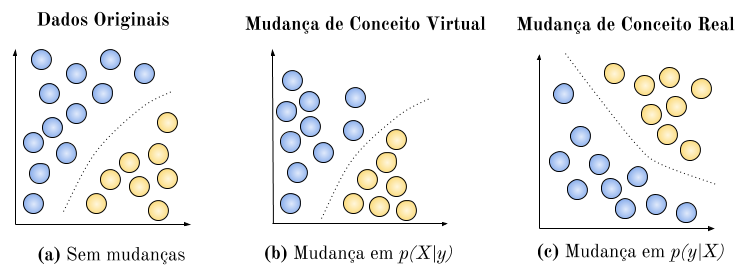
\includegraphics[scale=0.8]{imagens/concept_drift.png}
    \caption{Mudança de Conceito Virtual vs. Mudança de Conceito Real}
    \label{fig:real_and_virtual_concept_drift}
\end{center}
\end{figure}

Conforme \cite{Gama:2014:SCD:2597757.2523813}, as mudanças de conceito podem ocorrer de forma abrupta, gradual, incremental ou recorrente.
A Figura \ref{fig:concept_drift_patterns} ilustra estes padrões:

\begin{figure}[H]
\begin{center}
    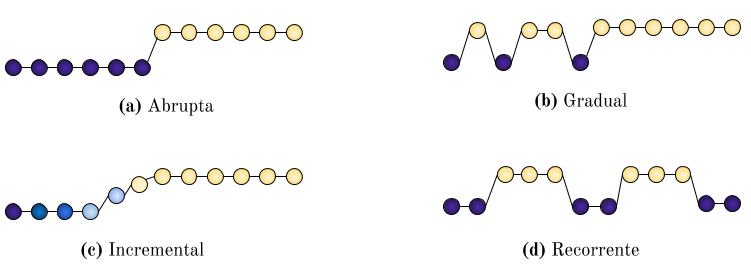
\includegraphics[scale=0.8]{imagens/concept_drift_patterns.png}
    \caption{Padrões de ocorrência de Mudanças de Conceito}
    \label{fig:concept_drift_patterns}
\end{center}
\end{figure}

Mudanças de conceito abruptas são alterações repentinas entre conceitos, como descrito na Figura \ref{fig:concept_drift_patterns} (a).
Por exemplo, o gênero literário preferido de um cliente pode mudar repentinamente de ficção científica para auto-ajuda.
Outro exemplo, é a troca de um sensor por outro com diferente calibração, em uma planta industrial química \cite{Gama:2014:SCD:2597757.2523813}. 

A mudança de conceito gradual representa uma transição mais lenta de um conceito para outro.
Isto é, durante a transição, são percebidos eventos de ambos os conceitos.
Pode-se considerar que o cliente, ao invés de subitamente passar a preferir livros de auto-ajuda, adquire interesse nestes ao longo do tempo.
Isto significa que ainda existe certo interesse em livros de ficção científica, mas, em paralelo, desenvolve-se uma crescente preferência por livros de auto-ajuda, que se tornará predominante.
A mudança de conceito gradual é representada na Figura \ref{fig:concept_drift_patterns} (b).

Mudanças de conceito incrementais apresentam conceitos intermediários durante a transição de um conceito para outro.
Para o exemplo utilizado, é como se o interesse literário variasse de ficção científica para ficção científica e aventura, 
de ficção científica e aventura para aventura e suspense, de aventura e suspense para suspense e auto-ajuda, e finalmente de suspense e auto-ajuda para apenas auto-ajuda.
Considerando a planta industrial química e os sensores, seria como se um sensor perdesse precisão ao longo do tempo. 
A Figura \ref{fig:concept_drift_patterns} (c) demonstra a mudança de conceito incremental. 

A mudança de conceito recorrente surge quando um conceito, previamente ativo, reaparece após determinado período de tempo.
Em nosso exemplo, considere que o cliente está atualmente interessado em livros de ficção científica.
Contudo, ele é presenteado com uma série de livros de auto-ajuda de um renomado autor.
Após ler toda a série, o cliente é premiado com descontos para livros de ficção científica e volta a lê-los.
A mudança de conceito recorrente está representada na Figura \ref{fig:concept_drift_patterns} (d).

O método de detecção proposto neste trabalho de mestrado busca identificar mudanças de conceito reais em fluxos contínuos de dados, independente do padrão de ocorrência destas.

Na subseção seguinte, será discutida a taxonomia do termo mudança de conceito e discriminada a expressão detecção de mudança de conceito de outras técnicas relacionadas.

\subsection{Taxonomia}

O fenômeno mudança de conceito tem sido estudado em diferentes comunidades de pesquisa, incluindo mineração de dados, 
aprendizado de máquina, estatística e recuperação de informação \cite{Zliobaite:2010}.
Contudo, o mesmo conceito pode ter diferentes nomeclaturas em cada comunidade.
Na Tabela \ref{tbl:taxonomy} são listados os termos correspondentes a mudança de conceito para cada área de pesquisa.

\begin{center} 
\begin{table}[H]
\label{tbl:taxonomy}
\begin{tabularx}{\textwidth}{|l|X|}
\cline{1-2}
\multicolumn{1}{|c|}{\textbf{Área}} & \multicolumn{1}{c|}{\textbf{Termos}}       \\ \cline{1-2}
Mineração de Dados                  & Mudança de Conceito                        \\ \cline{1-2}
Aprendizado de Máquina              & Mudança de Conceito, Mudança de Covariável \\ \cline{1-2}
Computação Evolucionária            & Ambiente Evolutivo, Ambiente em Mudança    \\ \cline{1-2}
IA e Robótica                       & Ambiente Dinâmico                          \\ \cline{1-2}
Estatísticas, Séries Temporais      & Não Estacionário                           \\ \cline{1-2}
Recuperação de Informação           & Evolução Temporal                          \\ \cline{1-2}
\end{tabularx}
\caption{Terminologia - Mudança de Conceito \cite{Zliobaite:2010}}
\end{table}
\end{center}

Outra fonte comum de equívocos são os termos Detecção de \textit{Outliers}, Detecção de Novidade, Detecção de \textit{Change Points} e Detecção de Mudança de Conceito.
Estes termos são, em muitos cenários, utilizados de forma indistinta.
Mas, para o contexto deste trabalho, é importante distingui-los.

De acordo com \cite{Chandola:2009:ADS:1541880.1541882}, a expressão Detecção de \textit{Outliers} refere-se a tarefa de encontrar padrões nos dados em desacordo com o comportamento esperado.

Ainda conforme \cite{Chandola:2009:ADS:1541880.1541882}, as técnicas para Detecção de Novidade têm como objetivo detectar padrões ainda não observados nos dados.
Diferentemente das técnicas para Detecção de \textit{Outliers}, as técnicas para Detecção de Novidade incorporam os novos padrões ao modelo de decisão.

% Entretanto, esse termo se distingue da detecção de \textit{outliers}, pois os novos padrões, geralmente, são incorporados ao modelo.
% Apesar de apresentarem definições próximas, a Detecção de Mudança de Conceito engloba a Detecção de Novidade e a extrapola, ao identificar 
% mudanças de conceito reais a partir do \textit{feedback} sobre a performance preditiva \cite{Gama:2010:KDD:1855075}.

% Esses padrões podem ser denominados como: \textit{outliers}, anomalias, observações discordantes, exceções, peculiaridades ou aberrações.
% Para \cite{Gama:2010:KDD:1855075}, exemplos esparsos e independentes, cujas características diferem muito daqueles que definem o modelo, 
% devem ser considerados como \textit{outliers}, pois não há garantia de que representem um conceito. 
% Em \cite{Aggarwal:2003:FCE:1315451.1315460}, os autores tipificam os \textit{outliers} como anomalias ou ruídos.
% As anomalias constituem um tipo especial de \textit{outlier}, que é de interesse dos analistas.
% Contudo, conforme \cite{Gama:2010:KDD:1855075}, é necessário um grupo conciso de exemplos para evidenciar o aparecimento de um novo conceito, ou novidade.

Por fim, as técnicas para Detecção de \textit{Change Points} identificam variações abruptas de valor, que podem representar transições entre estados, em séries temporais unidimensionais estacionárias \cite{Aminikhanghahi:2017:SMT:3086013.3086037}.

Na próxima subseção, detalharemos as principais técnicas para detecção de mudanças de conceito encontradas na literatura.

\subsection{Algoritmos para Detecção de Mudança de Conceito}

Os algoritmos para detecção de mudança de conceito são os responsáveis por identificar, de forma explícita, as referidas mudanças \cite{Gama:2014:SCD:2597757.2523813}.
Estes métodos caracterizam e quantificam as mudanças de conceito através da delimitação dos instantes ou intervalos de tempo em que as mudanças ocorrem \cite{Basseville:1993:DAC:151741}.

Essas técnicas podem ser divididas em duas categorias principais, conforme a dependência ou não de rotulação dos dados:
\begin{description}
    \item[Algoritmos Explícitos/Supervisionados] Dependem da rotulação dos dados por um especialista.
    Estes rótulos são utilizados no cálculo de medidas de performance como taxa de erro e acurácia, que são monitoradas ao longo do tempo.
    Mudanças de conceito são sinalizadas quando essas medidas atingem um limite previamente definido.

    \item[Algoritmos Implícitos/Não Supervisionados] Independem da rotulação por especialistas, 
    baseando-se em características dos próprios dados para sinalizar desvios.
    São mais propensos a alarmes falsos, mas a independência de rótulos os torna interessantes para contextos onde a obtenção desses é dispendiosa, demorada ou inviável.
\end{description}

Em sua pesquisa \cite{Gama:2014:SCD:2597757.2523813} categorizou os algoritmos supervisionados em três grupos principais:

\begin{description}
    \item[Métodos Baseados em Análise Sequencial] Avaliam, de forma sequenciada, os resultados das predições conforme tornam-se disponíveis (performance).
    Indicam a ocorrência de mudança de conceito quando um limite pré-definido é atingido.
    Os algoritmos \textit{Cumulative Sum (CUSUM)}, \textit{PageHinkley (PH)} \cite{Page:CUSUM:PageHinkley:1954} e \textit{Geometric Moving Average (GMA)} \cite{Roberts:2000:CCT:338441.338464}
    são representantes deste grupo.

    \item[Abordagens baseadas em Estatística] Identificam mudanças de conceito através da análise de parâmetros estatísticos como média e desvio padrão para os resultados das predições.
    Os métodos \textit{Drift Detection Method (DDM)} \cite{GamaMCR04}, 
    \textit{Early Drift Detection Method (EDDM)} \cite{EDDM}, 
    \textit{Exponentially Weighted Moving Average (EWMA)} \cite{Ross:2012:EWM:2076039.2076307} e 
    \textit{Reactive Drift Detection Method (RDDM)} \cite{Barros:RDDM:2017} são exemplos deste grupo.

    \item[Métodos baseados em Janelas] Geralmente, utilizam uma janela de tamanho fixo para sumarizar informações passadas e uma janela deslizante para sumarizar dados mais recentes.
    A mudança de conceito é detectada quando há uma diferença significativa entre as distribuições das janelas.
    Esta diferença é detectada a partir de testes estatísticos ou desigualdades matemáticas, considerando como hipótese nula a igualdade entre as distribuições.
    Os algoritmos 
    \textit{Adaptive Windowing (ADWIN)} \cite{BifetG07}, 
    \textit{SeqDrift} \cite{PearsSK14:SeqDrift:2014}, 
    \textit{HDDMA} e \textit{HDDMW} \cite{BlancoCRBDM15:HDDMA:HDDMW:2015}
    são membros desta família.
\end{description}

Os algoritmos implícitos também foram divididos em três grupos \cite{GONCALVES20148144}:

\begin{description}
    \item[Detecção de Novidade / Métodos de Agrupamento] 
    Utilizam a distância e/ou a densidade dos dados para detectar novos padrões.
    O algoritmo identifica exemplos suspeitos e os atribui a uma classe \textit{Desconhecido}, indicando a necessidade de uma avaliação adicional.
    As técnicas de agrupamento e detecção de \textit{outliers} são estratégias de implementação populares para estes algoritmos, 
    pois sintetizam os dados correntes e aplicam medidas de dissimilaridade para identificar novos padrões \cite{Ryu:Kantardzic:2012}.
    Os métodos 
    \textit{OLINDDA} \cite{Spinosa:2007:OCA:1244002.1244107},
    \textit{MINAS} \cite{Faria:2013:NDA:2480362.2480515},
    \textit{Woo} \cite{Ryu:Kantardzic:2012},
    \textit{DETECTNOD} \cite{Hashemi:Hayat:DETECTNOD:2010},
    \textit{ECSMiner} \cite{Masud:2011:CNC:1978259.1978529} e
    \textit{GC3} \cite{Sethi2016b:GC3} fazem parte deste grupo.
    
    \item[Monitoramento de distribuição multivariada]
    Monitoram diretamente a distribuição dos dados através de subconjuntos.
    Um subconjunto de treinamento tem sua distribuição sumarizada e armazenada, para ser utilizada como referência.
    A distribuição referência é comparada à distribuição do subconjunto atual e, havendo diferenças significativas, a mudança de conceito é sinalizada.
    Os algoritmos
    \textit{CoC} \cite{Lee:Magoules:CoC:2012},
    \textit{HDDDM} \cite{Ditzler:Polikar:HDDDM:2011},
    \textit{PCA-detect} \cite{Kuncheva:PCADetect:20085}
    são representantes deste grupo.

    \item[Monitoramento dependente de modelo]
    As técnicas elencadas nos grupos anteriores monitoram desvios na distribuição dos dados para indicar mudanças de conceito.
    Essencialmente, esses métodos assumem que alterações na distribuição, $P(X)$, implicarão mudanças na performance do classificador, $p(c|X)$.
    Apesar de permitir a aplicação de qualquer tipo de classificador, essa presunção leva a uma maior quantidade de falsos positivos.
    As técnicas dependentes de modelo, por sua vez, restringem-se aos classificadores probabilísticos,
    o que permite realizar a detecção de mudanças de conceito através do monitoramento das probabilidades a posteriori \cite{Zliobaite:2010}.
    A utilização destas probabilidades diminui a incidência de falsos positivos e torna o processo computacionalmente eficiente, 
    pois apenas um único fluxo univariado de valores é observado.
    Os métodos 
    \textit{A-distance} \cite{Dredze:ADistance:2010585},
    \textit{CDBD} \cite{Lindstrom:CDBD:2013} e
    \textit{Margin} \cite{Dries:Margin:2009} participam deste grupo.
\end{description}

Por fim, a Tabela \ref{tbl:abordagens} sumariza as categorias, os grupos e as respectivas técnicas mencionadas nesta seção.

% Please add the following required packages to your document preamble:
% \usepackage{graphicx}
\begin{table}[!ht]
    \centering
    \resizebox{\textwidth}{!}{%
    \begin{tabular}[t]{@{}lllll@{}}
    \hline \\
    Algoritmos Explícitos/Supervisionados     & Métodos Baseados em Análise Sequencial        & \begin{tabular}[t]{@{}l@{}} Cumulative Sum (CUSUM) \\ PageHinkley (PH) \cite{Page:CUSUM:PageHinkley:1954} \\ Geometric Moving Average (GMA) \cite{Roberts:2000:CCT:338441.338464}\end{tabular}                                                                                                                        &  &  \\ \\
                                              & Abordagens baseadas em Estatística            & \begin{tabular}[t]{@{}l@{}} Drift Detection Method (DDM) \cite{GamaMCR04} \\  Early Drift Detection Method (EDDM) \cite{EDDM} \\  Exponentially Weighted Moving Average (EWMA) \cite{Ross:2012:EWM:2076039.2076307} \\ Reactive Drift Detection Method (RDDM) \cite{Barros:RDDM:2017} \end{tabular}                                                                &  &  \\ \\
                                              & Métodos baseados em Janelas                   & \begin{tabular}[t]{@{}l@{}} Adaptive Windowing (ADWIN) \cite{BifetG07} \\   SeqDrift \cite{PearsSK14:SeqDrift:2014} \\   HDDMA/HDDMW \cite{BlancoCRBDM15:HDDMA:HDDMW:2015} \end{tabular}                                                                                            &  &  \\ \\
    
    Algoritmos Implícitos/Não Supervisionados & Detecção de Novidade / Métodos de Agrupamento & \begin{tabular}[t]{@{}l@{}} OLINDDA \cite{Spinosa:2007:OCA:1244002.1244107} \\   MINAS \cite{Faria:2013:NDA:2480362.2480515} \\   Woo \cite{Ryu:Kantardzic:2012} \\   DETECTNOD \cite{Hashemi:Hayat:DETECTNOD:2010} \\   ECSMiner \cite{Masud:2011:CNC:1978259.1978529} \\   GC3 \cite{Sethi2016b:GC3} \end{tabular} &  &  \\ \\
                                              & Monitoramento de distribuição multivariada    & \begin{tabular}[t]{@{}l@{}} CoC \cite{Lee:Magoules:CoC:2012} \\ HDDDM \cite{Ditzler:Polikar:HDDDM:2011} \\ PCA-detect \cite{Kuncheva:PCADetect:20085} \end{tabular}                                       &  &  \\ \\
                                              & Monitoramento dependente de modelo            & \begin{tabular}[t]{@{}l@{}} A-distance \cite{Dredze:ADistance:2010585} \\ CDBD \cite{Lindstrom:CDBD:2013} \\ Margin \cite{Dries:Margin:2009} \end{tabular}                                                                                        &  &  \\ \\
    \hline
    \end{tabular}%
    }
    \caption{Sumário - Abordagens de detecção \cite{Sethi:2017:RDC:3096751.3096864}}
    \label{tbl:abordagens}
\end{table}

O algoritmo desenvolvido neste projeto de mestrado enquadra-se na categoria de algoritmos implícitos ou não supervisionados, mais especificamente no grupo \textit{Detecção de Novidades / Métodos de Agrupamento}.
Na próxima seção, abordaremos as ferramentas utilizadas para implementação da técnica e sua validação.

\subsection{Ferramentas}

Nesta seção, os frameworks \textit{Massive Online Analysis} (MOA) e \textit{Tornado} serão apresentados.
Estes frameworks possibilitam a implementação e a análise - perante o estado da arte - de algoritmos para detecção de mudanças de conceito.
Ambos permitem a avaliação entre técnicas e a utilização de diferentes fontes de dados.

\subsection{MOA}

O \textit{MOA – Massive Online Analysis}\footnote{https://moa.cms.waikato.ac.nz/} é, atualmente, o principal framework para mineração de dados em fluxos contínuos.
O projeto é de código-aberto\footnote{https://github.com/Waikato/moa} e apresenta uma comunidade bastante ativa e crescente \cite{Bifet:2010:MMO:1756006.1859903}.
A aplicação é composta por uma ampla coleção de algoritmos da área de aprendizado de máquina: classificação, regressão, agrupamento, busca por padrões, detecção de \textit{outliers}, detecção de mudanças de conceito e sistemas de recomendação.
Além de conter ferramentas para avaliação destes.
Apresenta relação com o projeto WEKA \cite{Hall:2009:WDM:1656274.1656278}, sendo também desenvolvido em Java, o que permite a sua execução nos principais sistemas operacionais.

O MOA divide suas funcionalidades em tarefas (\textit{tasks}).
As principais tarefas incluem:
produção de fluxos de dados,
treino de classificadores,
aplicação de algoritmos de agrupamento,
análise de algoritmos para detecção de \textit{outliers} e de \textit{concept drift}, dentre outras.
As tarefas podem ser executadas a partir da interface gráfica (GUI) ou por linha de comando.
A tela principal da aplicação é demonstrada na Figura \ref{fig:moa}.
Através da interface gráfica é possível executar múltiplas tarefas de forma concorrente, 
controlar suas execuções e visualizar os resultados parciais.

\begin{figure}[H]
\begin{center}
    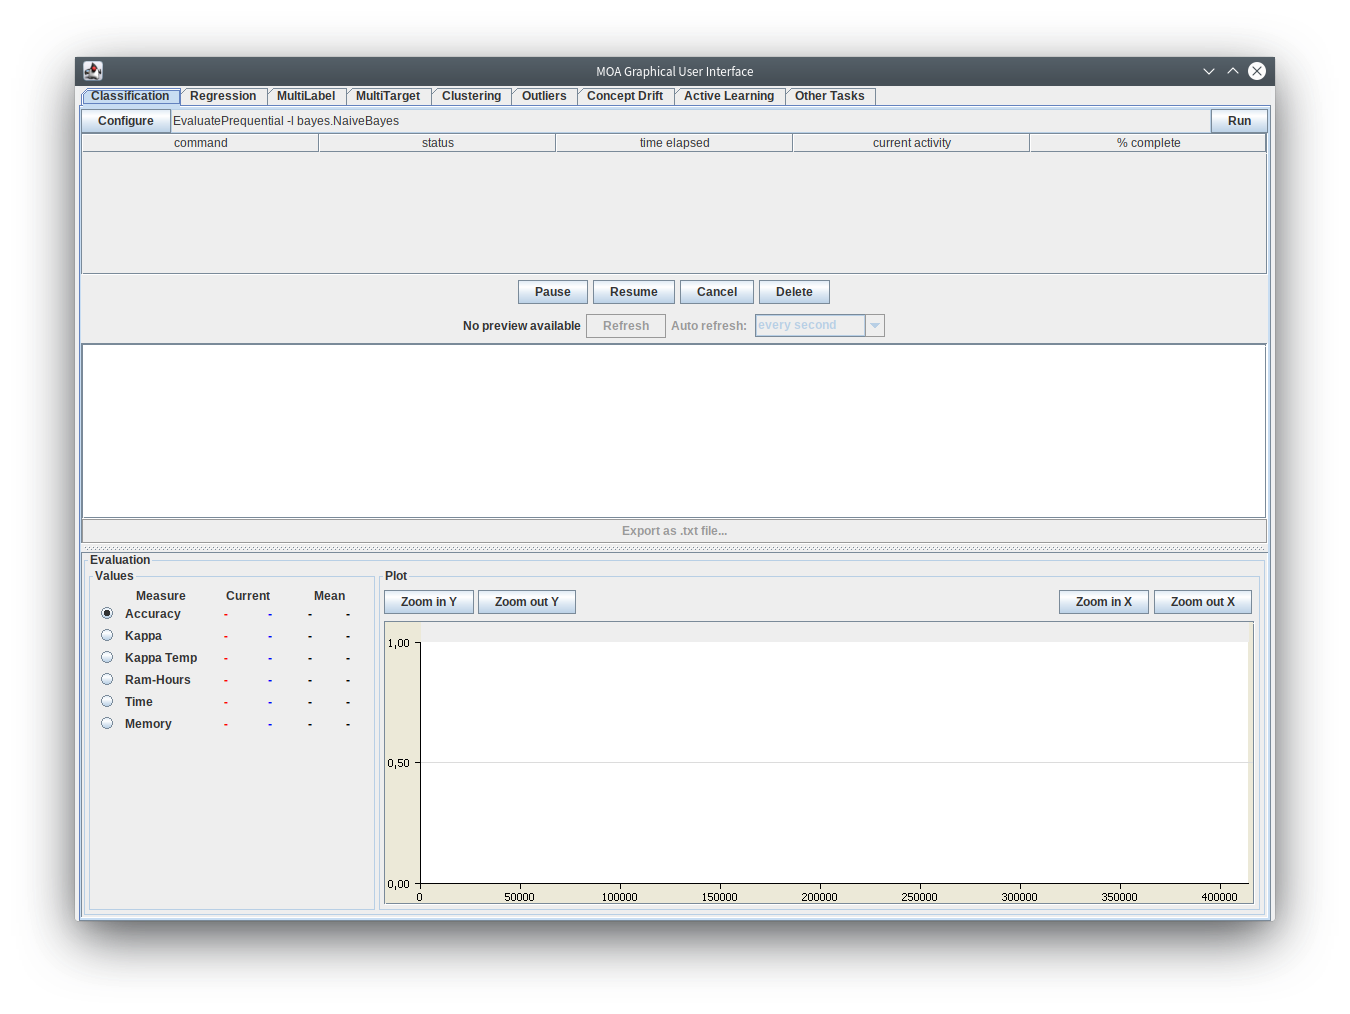
\includegraphics[scale=0.4]{imagens/moa.png}
    \caption{MOA - Tela Inicial}
    \label{fig:moa}
\end{center}
\end{figure}

A aplicação é capaz de ler arquivos em formato \textit{ARFF}, populares por serem utilizados no projeto WEKA \cite{Hall:2009:WDM:1656274.1656278}.
A ferramenta também permite a produção de fluxos de dados dinamicamente, através de geradores.
Alguns dos geradores de fluxo disponíveis no MOA são:
\textit{Random Trees} \cite{Domingos:2000:MHD:347090.347107}
\textit{SEA} \cite{Street:2001:SEA:502512.502568}, 
\textit{STAGGER} \cite{Schlimmer1986}, 
\textit{Rotating Hyperplane} \cite{Wang:2003:MCD:956750.956778},
\textit{Random RBF}, 
\textit{LED} \cite{Gama:2003:ADT:956750.956813}, 
\textit{Waveform} \cite{Gama:2003:ADT:956750.956813}, 
 e \textit{Function} \cite{Jin:2003:EDT:956750.956821}.

Outra funcionalidade importante do framework é a possibilidade de adicionar mudanças de conceito a fluxos estacionários existentes.
Isto é feito através de uma função sigmóide, que modela o evento de mudança de conceito como uma combinação balanceada de duas distribuições homogêneas, 
que caracterizam os conceitos-alvo antes e depois da mudança \cite{bifet2009data}.
Além destes conceitos, o usuário também pode definir o momento da mudança e a sua duração \cite{Bifet:2010:MMO:1756006.1859903}.

Os principais métodos para detecção de mudança de conceito propostos na literatura estão disponíveis no MOA.
O framework também permite a utilização de classificadores do WEKA \cite{Hall:2009:WDM:1656274.1656278} combinados aos detectores.
A janela para configuração de um detector é demonstrada na Figura \ref{fig:moa_detector}.

\begin{figure}[H]
\begin{center}
    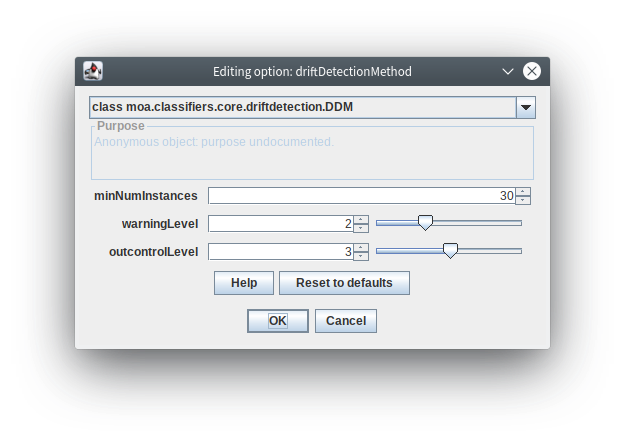
\includegraphics[scale=1]{imagens/detector.png}
    \caption{MOA - Configuração detector}
    \label{fig:moa_detector}
\end{center}
\end{figure}

A arquitetura do framework é modular, o que permite aos usuários implementar novas tarefas com pouco esforço.
Por exemplo, para criar um novo detector, basta estender a classe abstrata \texttt{moa.classifiers.core.driftdetection.AbstractChangeDetector} e implementar o algoritmo desejado.
A janela de configuração para o detector (similar a \ref{fig:moa_detector}) é criada dinamicamente, a partir dos atributos da classe.

O MOA dispõe de diversas classes para avaliação de técnicas de aprendizado de máquina. 
Para este trabalho, destacam-se as classes \texttt{DriftDetectionMethodClassifier} e \texttt{BasicConceptDriftPerformanceEvaluator}, 
que realizam a análise de algoritmos para detecção de mudança de conceito.
A classe \texttt{DriftDetectionMethodClassifier} permite avaliar técnicas de detecção que encapsulam um classificador.
Por sua vez, a classe \texttt{BasicConceptDriftPerformanceEvaluator} avalia a performance das técnicas de detecção diretamente, 
sem a necessidade de um classificador.
Estes avaliadores e os seus indicadores serão detalhados juntamente com os resultados dos experimentos iniciais, na Seção \ref{experimentos_iniciais}.

\subsection{Tornado}

O Tornado é um framework para avaliação de algoritmos de detecção de mudança de conceito \cite{Pesaranghader:Tornado}.
O projeto é desenvolvido na linguagem Python e seu código está disponível\footnote{https://github.com/alipsgh/tornado}.
O framework diferencia-se do MOA por apresentar um cenário de avaliação específico: 
analisar a execução, em paralelo, de pares (classificador, detector de mudança de conceito), 
para identificar o par ótimo ao longo do tempo, em relação ao fluxo de dados.

\begin{figure}[H]
\begin{center}
    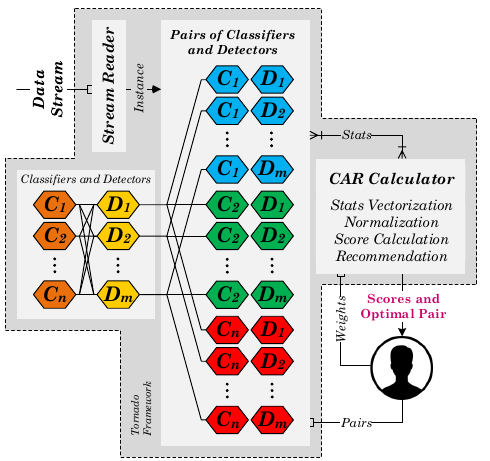
\includegraphics[scale=0.75]{imagens/tornado.png}
    \caption{Framework Tornado \cite{Pesaranghader:Tornado}.}
    \label{fig:tornado}
\end{center}
\end{figure}

Conforme apresentado na Figura \ref{fig:tornado}, os principais componentes do framework são: 
\textit{Stream Reader}, \textit{Classifiers}, \textit{Detectors}, \textit{Classifier-Detector Pairs} e \textit{CAR Calculator}.
A entrada de dados é composta por um fluxo (\textit{Stream}), uma lista de pares (classificador, detector) e um vetor com pesos.

O componente \textit{Stream Reader} lê instâncias a partir do fluxo e as envia, uma a uma, para o par (classificador, detector), para construção do modelo.
Os modelos são construídos de forma incremental. Por seguir a abordagem \textit{prequential}, cada instância é primeiramente utilizada para testes e depois como treinamento.
Simultaneamente, os classificadores enviam suas estatísticas (taxas de erro ou resultados das predições) aos detectores, para que a mudança de conceito possa ser sinalizada.
Por fim, o componente \textit{CAR Calculator} calcula uma pontuação para cada par, considerando taxas de erro, atraso para detecção da mudança de conceito, falsos positivos, falsos negativos, quantidade de memória utilizada e tempo de execução \cite{Pesaranghader:Tornado}.
O framework apresenta ao usuário o par com maior pontuação. Este par, contudo, pode mudar devido ao aprendizado incremental ou à mudança de conceito.
A Figura \ref{fig:tornado_out2} apresenta um resultado obtido através do framework.

\begin{figure}[H]
\begin{center}
    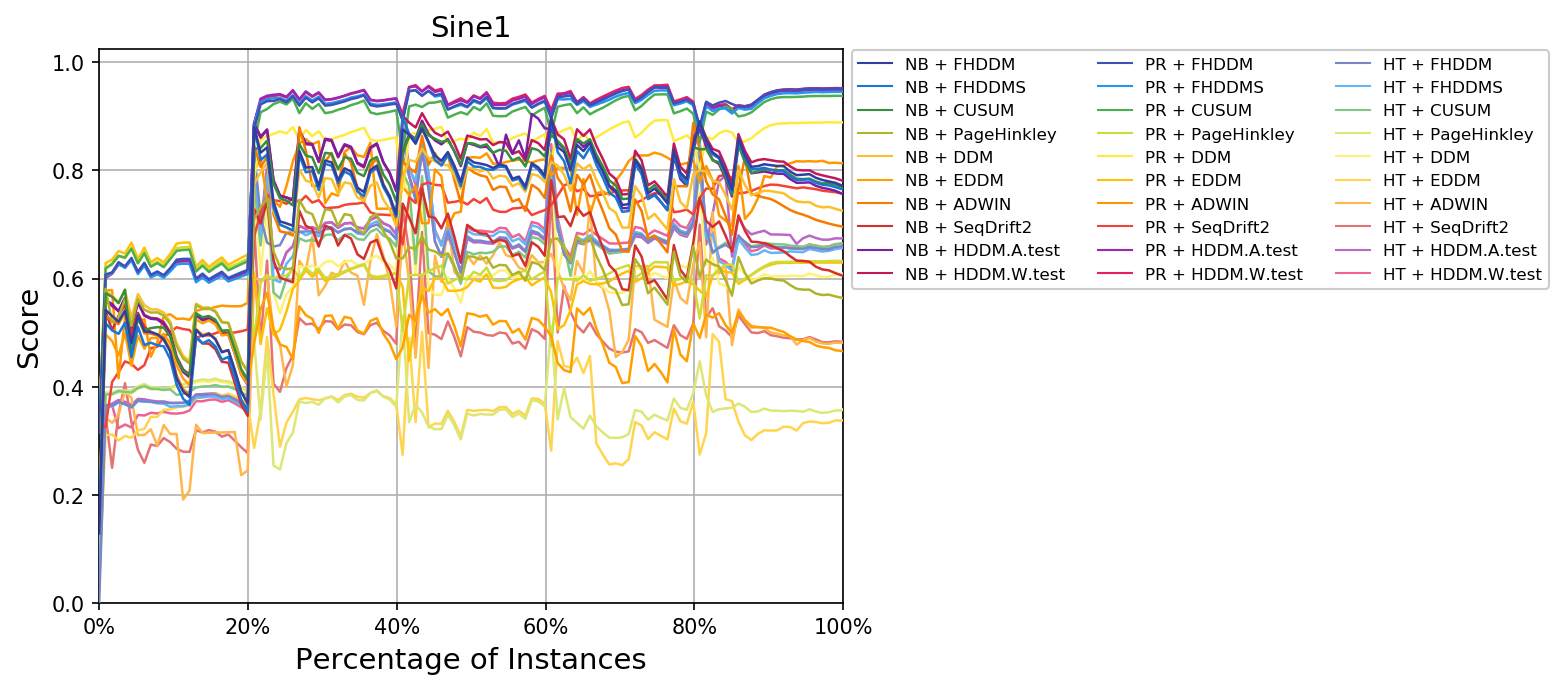
\includegraphics[scale=0.6]{imagens/tornado_out2.png}
    \caption{Tornado - Resultado para múltiplos pares \cite{Pesaranghader:Tornado}}
    \label{fig:tornado_out2}
\end{center}
\end{figure}

Neste trabalho, o algoritmo proposto foi implementado e testado nas duas ferramentas apresentadas.
Os detalhes de implementação e os resultados desses testes são discutidos na Seção \ref{experimentos_iniciais}.
A seguir, as redes de função de base radial serão detalhadas.

\section{Redes de Função de Base Radial}

As Redes de Função de Base Radial (RBF \textit{networks}) são aproximadoras universais de funções.
As RBFs têm como principal diferença em relação às outras redes neurais, a forma de ativação.
Nessas redes, este processo é feito através do cálculo da distância entre os vetores de entrada e os centros estabelecidos \cite{Braga:RedesNeuraisTeoriaAplicacoes}.

Em sua forma básica, a arquitetura de uma rede do tipo RBF é composta por três camadas: 
uma camada de entrada, uma intermediária e uma de saída \cite{Rojas:1996:NNS:235222}. 
A camada intermediária (oculta) de uma RBF utiliza funções de base radiais para agrupar os dados de entrada em clusters, 
transformando padrões de entrada não linearmente separáveis em um conjunto de saídas linearmente separáveis. 
A camada de saída classifica os padrões recebidos através da combinação linear das saídas das funções \cite{Braga:RedesNeuraisTeoriaAplicacoes}.
A Figura \ref{fig:rbg_arq} demonstra essa arquitetura.

\begin{figure}[H]
\begin{center}
    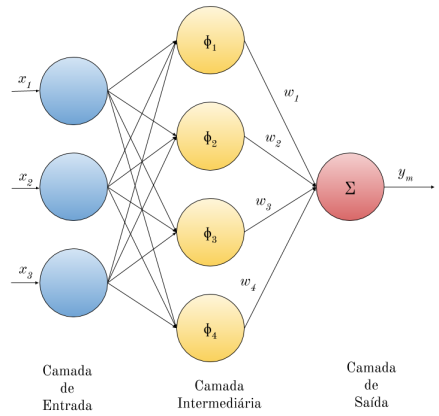
\includegraphics[scale=1]{imagens/rbf_arq.png}
    \caption{Arquitetura RBF}
    \label{fig:rbg_arq}
\end{center}
\end{figure}

Na literatura, a função de base radial Gaussiana (Eq. \ref{eq:gaussiana}) é uma das mais utilizadas para camada intermediária.

\begin{equation} \label{eq:gaussiana}
    f(x)=e^{-{\frac {v^{2}}{2\sigma^{2}}}}
\end{equation}

Na equação \ref{eq:gaussiana}, $v = \lVert x - t_i \rVert$ é dado pela distância euclidiana, onde $x$ é o valor de entrada da rede, 
enquanto $t_i$ e $\sigma$ correspondem respectivamente ao centro e a largura da função radial. 
Dessa maneira, a resolução de um determinado problema por uma rede do tipo RBF consiste na resolução das funções \ref{eq:rbf1} e
\ref{eq:rbf2}, obtendo o sistema \ref{eq:rbf3}.

\begin{equation} \label{eq:rbf1}
    f(x)=\sum _{{i=1}}^{N}w_{ij}\varphi (||{\mathbf  {x}}-{\mathbf  {t}}_{i}||)
\end{equation}

\begin{equation} \label{eq:rbf2}
    y_i=\sum _{{i=1}}^{N}w_{ij}\phi (||{\mathbf  {x}}-{\mathbf  {t}}_{i}||) + w_{j_0}
\end{equation}

\begin{equation} \label{eq:rbf3}
\begin{bmatrix}
    \varphi (||{{x_1}}-{{t}}_{1}||) & \varphi (||{{x_1}}-{{t}}_{2}||) & \dots & \varphi (||{{x_1}}-{{t}}_{N}||) \\
    \varphi (||{{x_2}}-{{t}}_{1}||) & \varphi (||{{x_2}}-{{t}}_{2}||) & \dots & \varphi (||{{x_2}}-{{t}}_{N}||) \\
    \hdotsfor{5} \\
    \varphi (||{{x_N}}-{{t}}_{1}||) & \varphi (||{{x_N}}-{{t}}_{2}||) & \dots & \varphi (||{{x_N}}-{{t}}_{N}||)
\end{bmatrix}
\begin{bmatrix}
    w_1 \\
    w_2 \\
    \vdots \\
    w_N \\
\end{bmatrix}
=
\begin{bmatrix}
    y_1 \\
    y_2 \\
    \vdots \\
    y_N \\
\end{bmatrix}
\end{equation}

onde $w_{ij}$ são os pesos de cada conexão, $\phi$ é a matriz de interpolação originada do conjunto de $N$ funções
de base radial aplicadas nas entradas $x$ e dos seus respectivos centros $t_i$,
$w_{j_0}$ representa o bias, $\varphi (||{{x}}-{{t}}_{i}||)$ é o conjunto de $N$ funções de base radial,
$||\ldots||$ é a norma euclidiana e $y$ são as saídas geradas pela rede.

As camadas inicial e intermediária e suas propriedades de agrupamento são utilizadas como base para o algoritmo de detecção de mudança de conceito 
proposto neste projeto de mestrado. 

\section{Trabalhos Relacionados}

Além das referências básicas apresentadas neste capítulo, foi realizada uma pesquisa na literatura visando identificar trabalhos também 
que propõem a identificação de mudanças de conceito em fluxos contínuos de dados através da aplicação de redes de função de base radial
ou que apliquem técnicas similares.

Em \cite{Jianping:Venkateswarlu:RBF:SpeakerIdentification} redes de função de base radial, utilizando funções gaussianas, são utilizadas para detecção de novidades.
A técnica proposta atua sobre cenários estacionários, mais especificamente o problema de identificação de falas.
Durante a preparação da rede, o algoritmo \textit{k-means} é utilizado para definir os centros e as matrizes de covariância.

Roberts e Penny \cite{Roberts:Penny:Novelty:Confidence} propõem  um método para detecção de novidade baseado no monitoramento das taxas de erro e confiança, 
utilizando um comitê de redes de função de base radial. 
Cada rede é inicializada com um vetor de pesos diferente.
A taxa de erro final é calculada a partir da matriz de covariância de erro do cômite criado.
Esta abordagem foi testada na classificação de pacientes com problemas de tremor muscular.

As redes de função de base radial também foram aplicadas para detecção de anomalias \cite{Bazargani2018RadialBF}.
Neste trabalho, às funções de perda (\textit{loss}) das redes são modificadas, 
tornando-as classificadores para uma única classe. 
Estas modificações permitem às redes identificar exemplos divergentes dos padrões conhecidos.

Este projeto de mestrado se diferencia dos trabalhos mencionados por utilizar apenas as camadas de entrada e intermediária das redes de função de base radial para detecção de mudanças de conceito.
Além disso, etapas como a escolha dos centros e o cálculo do tamanho do raio são realizadas de forma dinâmica, tornando possível a sua aplicação em cenários com fluxos contínuos de dados.

\section{Considerações Finais}

Neste capítulo foram apresentados os principais conceitos para a execução deste trabalho. 
Foram discutidas noções sobre a aplicação de técnicas de aprendizado a fluxos contínuos de dados,
o fenômeno mudança de conceito e suas técnicas de detecção e ferramentas,
as redes de função de base radial e, por fim, os principais trabalhos relacionados.
No próximo capítulo, o plano de pesquisa será detalhado.

\xchapter{Plano de Pesquisa}{} \label{plano_pesquisa}
\section{Considerações Iniciais}

\todo{Daqui}

Este capítulo descreve como a pesquisa proposta neste mestrado será desenvolvida para permitir que Redes de Função de Base Radial sejam aplicadas para detecção de mudanças de conceito em Fluxos Contínuos de Dados.
Espera-se que com a utilização das camadas inicial e intermediária das redes RBF e suas propriedades de agrupamento, seja possível detectar mudanças de conceito de forma eficiente e sem requerer a manutenção de estados prévios.
A seguir, são apresentados detalhes sobre cada etapa do desenvolvimento do projeto.

\section{Descrição do Problema}

O fenômeno Mudança de Conceito pode ser definido a partir do teorema de Bayes para probabilidades posteriores.
Seja $X$ um vetor de entrada e $Y$ a classe alvo,
a decisão de classificar $X$ como $Y$ dependerá da probabilidade posterior da classe, dada por:

\begin{equation} \label{eq:gaussiana}
    P(Y |X) = \frac{P(Y)P(X|Y)}{P(X)}
\end{equation}

onde $P(Y|X)$ é a probabilidade de $Y$ para a entrada $X$, $P(X|Y)$ é a distribuição condicional da classe para as variáveis da entrada $X$ e 
$P(Y)$ é a probabilidade a priori da classe e $P(X)$ é a probibilidade a priori do vetor de entrada $X$.

Na presença de mudança de conceito, a probabilidade posterior $P(Y|X)$ varia ao longo do tempo, isto é $P_{t_0}(Y|X)$ pode ser diferente de $P_{t_1}(Y|X)$.
Em outras palavras, os limites de decisão do classificador se alteram ao longo do tempo.

Considerando que redes de função de base radial apresentam em suas camadas inicial e intermediária características de agrupamento, 
este projeto de mestrado visa comprovara hipótese que redes RBF podem detectar mudanças de conceito em fluxos contínuos de dados, 
em tempo de execução, sem requerer a manutenção de estados prévios, de forma ágil e com precisão satisfatória.

Para exemplificar a execução desta proposta de mestrado, considere \ldots

\section{Atividades de Pesquisa}
\blindtext

\section{Considerações Finais}
\blindtext

\xchapter{Experimentos Iniciais}{} \label{experimentos_iniciais}
\section{Considerações Iniciais}
\blindtext

\section{Configuração dos Experimentos}
\blindtext

\section{Método de Pettitt}
\blindtext

\section{Redes de Função de Base Radial}
\blindtext

\section{Considerações Finais}
\blindtext


%% Parte pos-textual
\backmatter

% Bibliografia
% É aconselhável utilizar o BibTeX a partir de um arquivo, digamos "biblio.bib".
% Para ajuda na criação do arquivo .bib e utilização do BibTeX, recorra ao
% BibTeXpress em www.cin.ufpe.br/~paguso/bibtexpress
\bibliographystyle{abntex2-alf}
\bibliography{biblio}

% Apendices
% Comente se naoo houver apendices
%\appendix

%\xchapter{Exemplo de Ap\^endice}{} %sem preambulo
%\lipsum
% Eh aconselhavel criar cada apendice em um arquivo separado, digamos
% "apendice1.tex", "apendice.tex", ... "apendiceM.tex" e depois
% inclui--los com:
%\xchapter{Decomposição das séries temporais}{} %sem preambulo
\label{apendice1}
\section{Considerações Iniciais}
Neste apêndice consta as 40 séries temporais utilizadas nos experimentos mostrados no Capitulo \ref{experimentos}. As séries foram divididas em 4 tipos conforme a Tabela \ref{series}, onde o tipo representa um conjunto de 10 séries senoide ou cossenoide, sendo acrescida de ruído ou acrescida de ruído e tendência.
Nas imagens são representadas, a séries original,   seu componente determinístico e seu componente estocástico, os quais foram extraídos após a decomposição.
\section{Séries TIPO 1}
10 séries cossenoide com ruído ao longo da série.
\graphicspath{{imagens/}}
\begin{figure}[H]
\begin{center}
  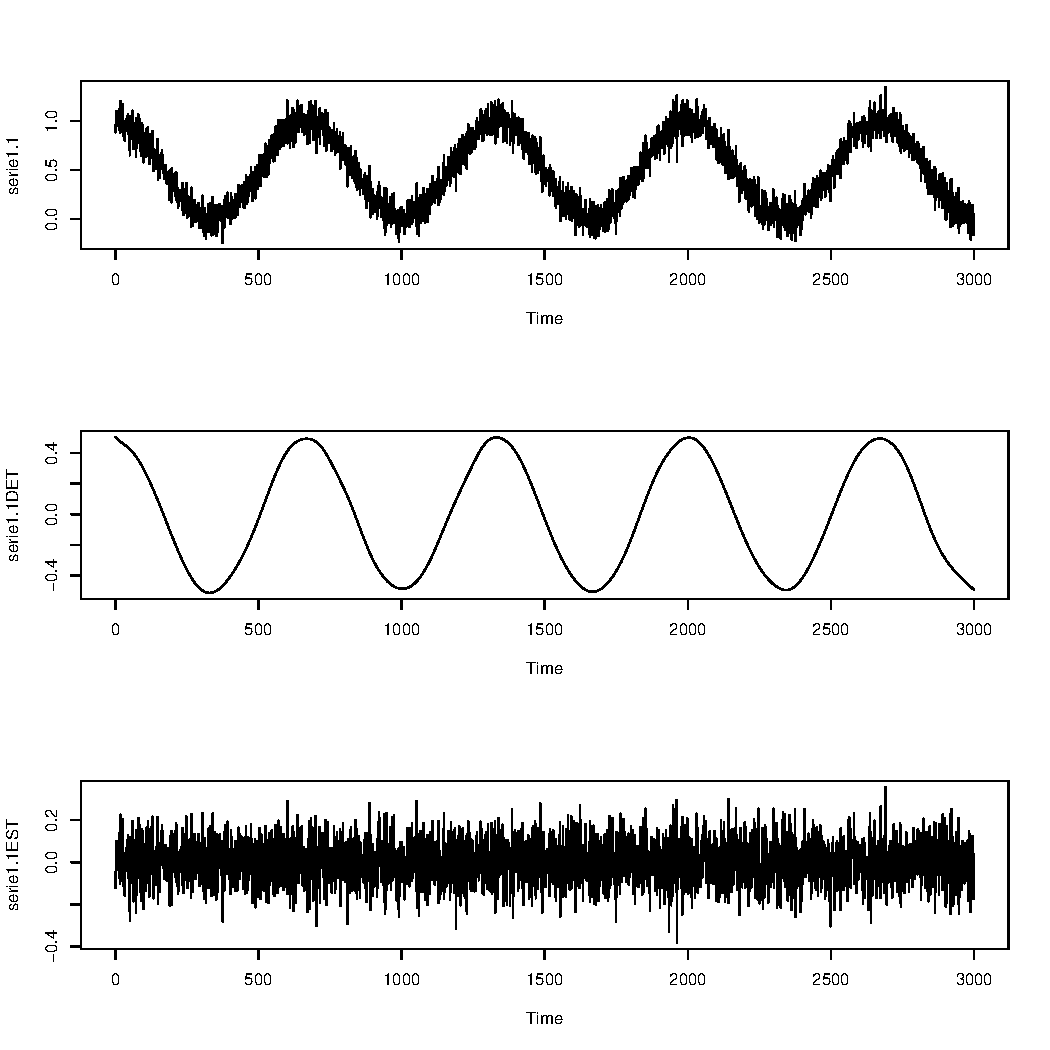
\includegraphics[scale=0.43]{serie1_1.pdf} \quad
  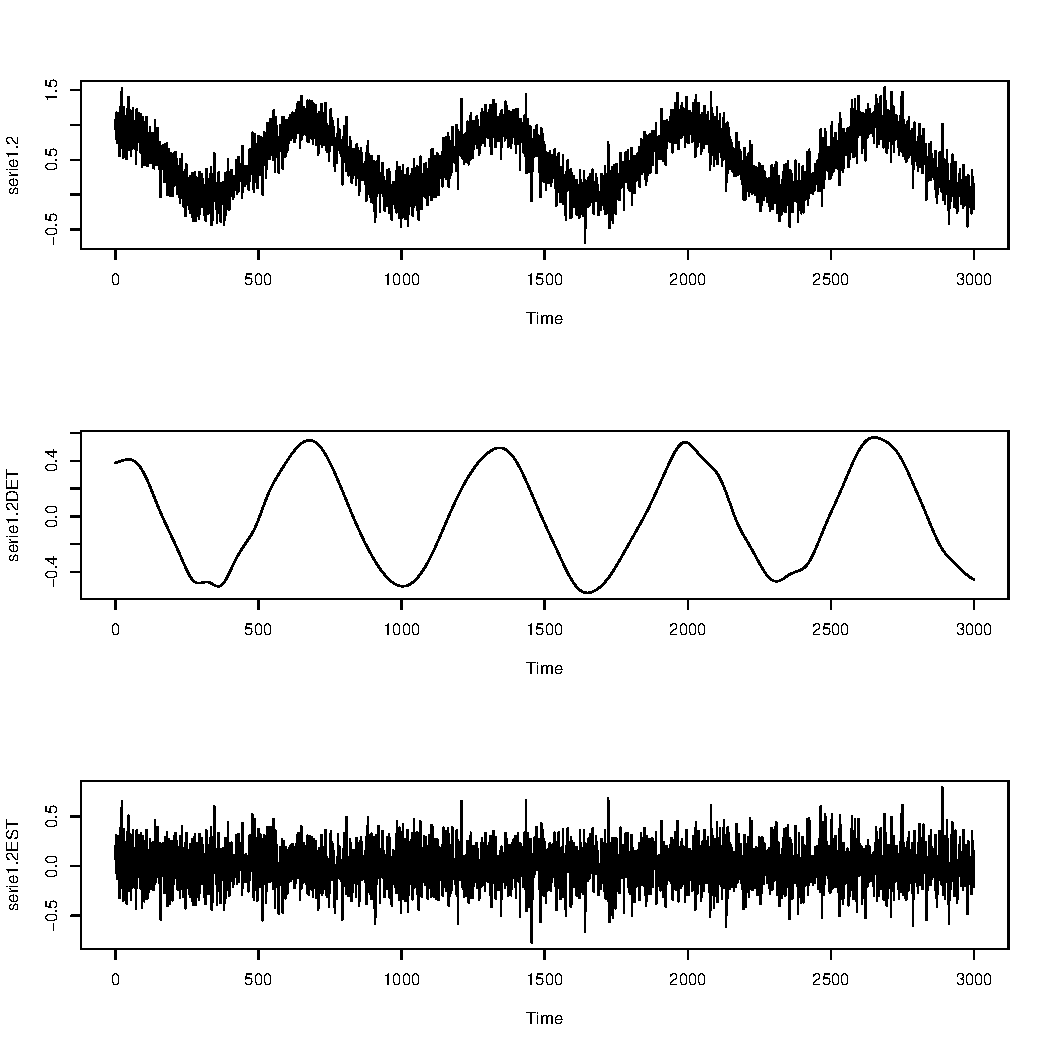
\includegraphics[scale=0.43]{serie1_2.pdf}
  \caption{Série 1.1 e Série 1.2}

\end{center}
\end{figure}

\graphicspath{{imagens/}}
\begin{figure}[H]
\begin{center}
  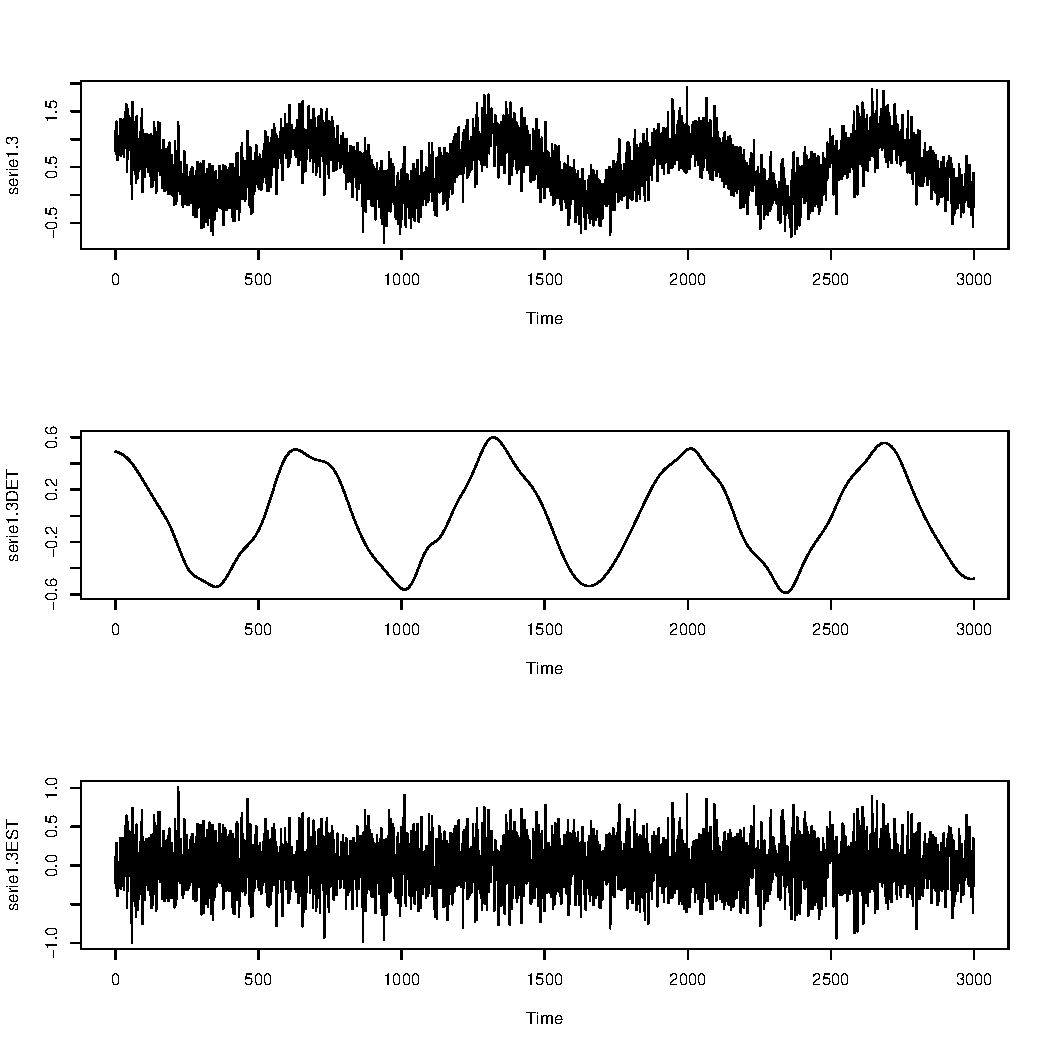
\includegraphics[scale=0.43]{serie1_3.pdf} \quad
  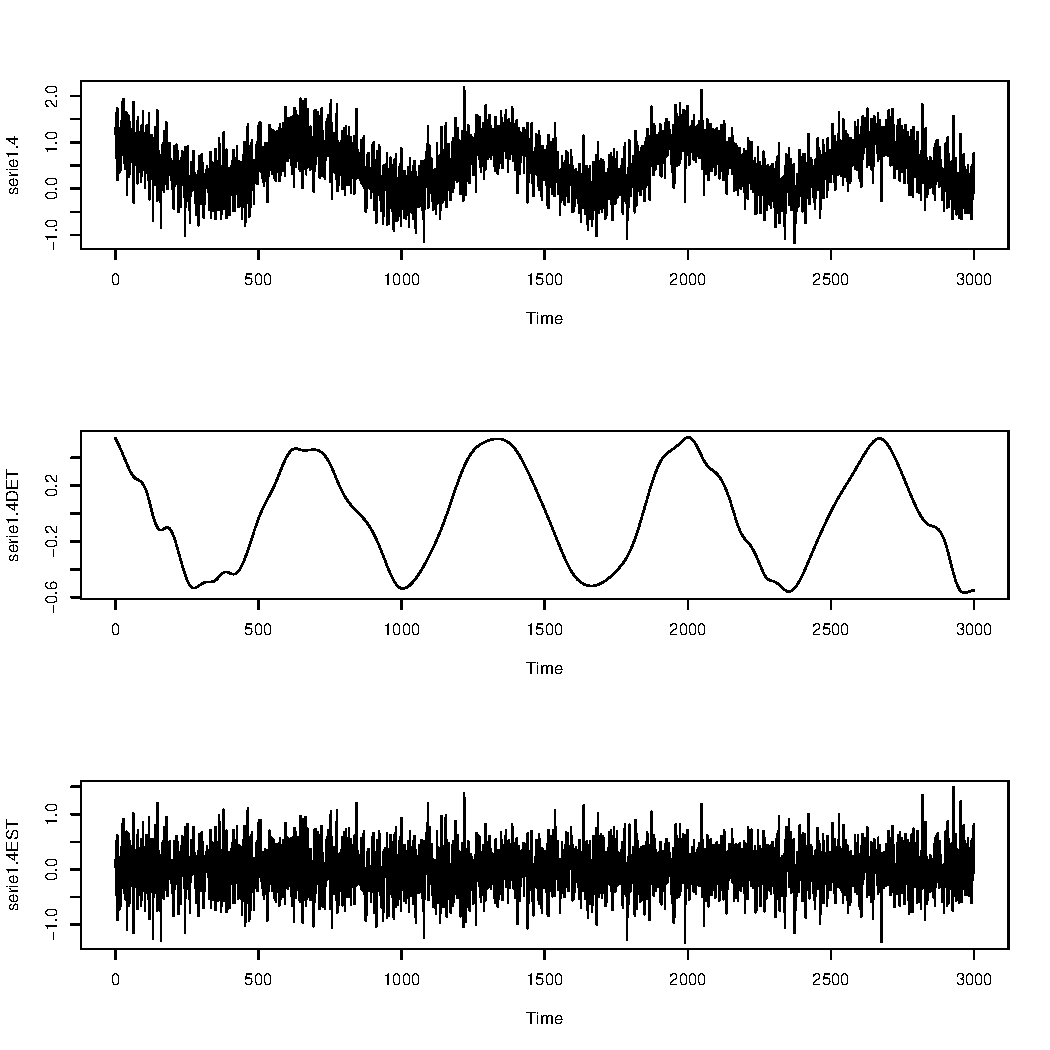
\includegraphics[scale=0.43]{serie1_4.pdf}
  \caption{Série 1.3 e Série 1.4}

\end{center}
\end{figure}

\graphicspath{{imagens/}}
\begin{figure}[H]
\begin{center}
  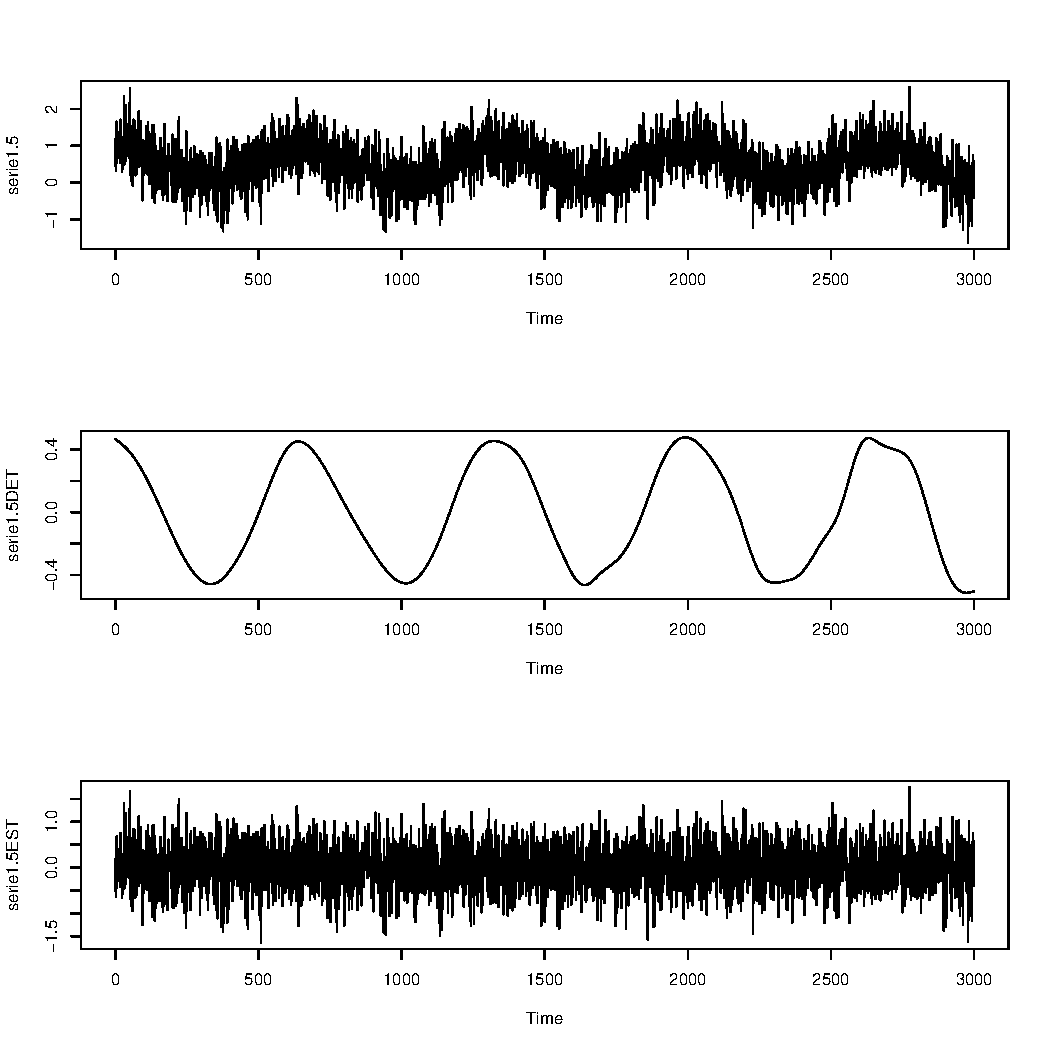
\includegraphics[scale=0.43]{serie1_5.pdf} \quad
  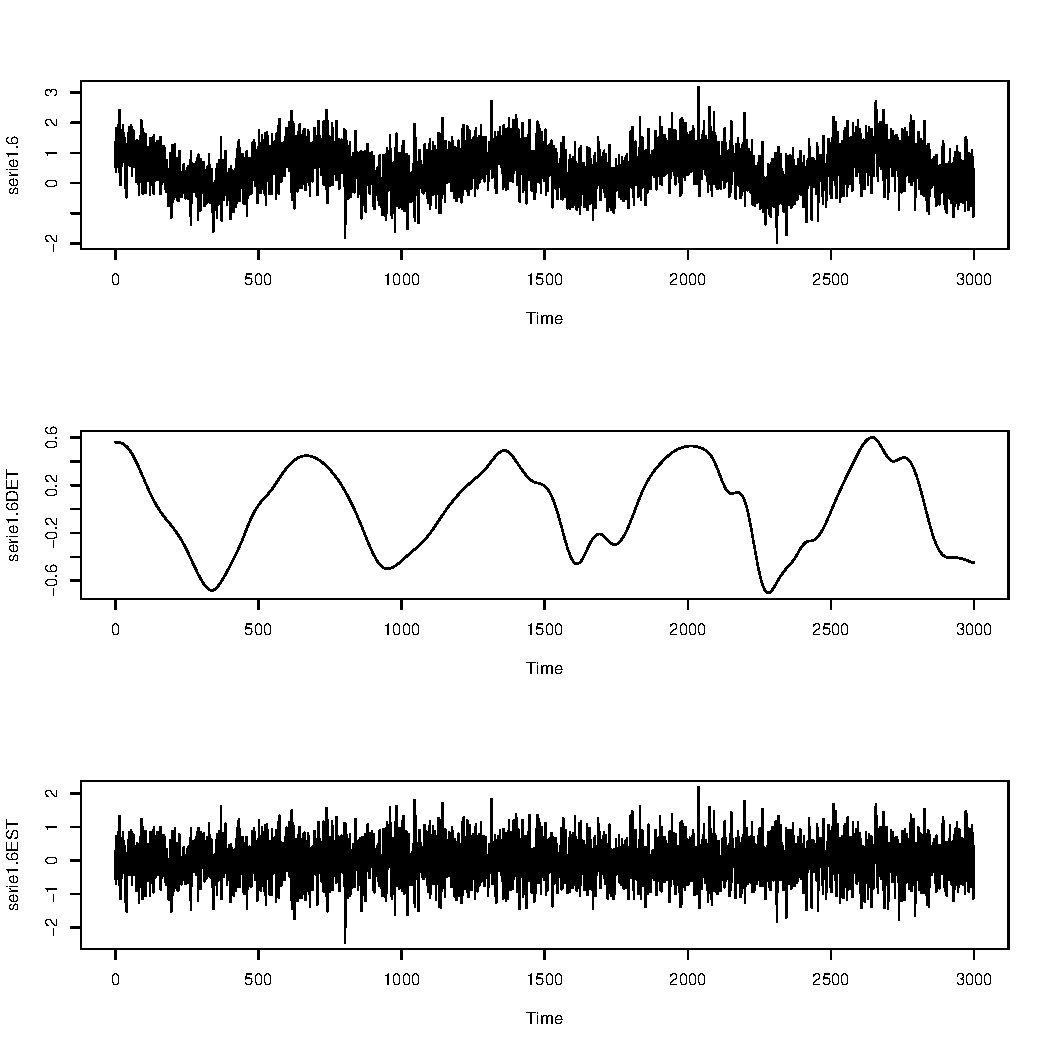
\includegraphics[scale=0.43]{serie1_6.pdf}
  \caption{Série 1.5 e Série 1.6}

\end{center}
\end{figure}

\graphicspath{{imagens/}}
\begin{figure}[H]
\begin{center}
  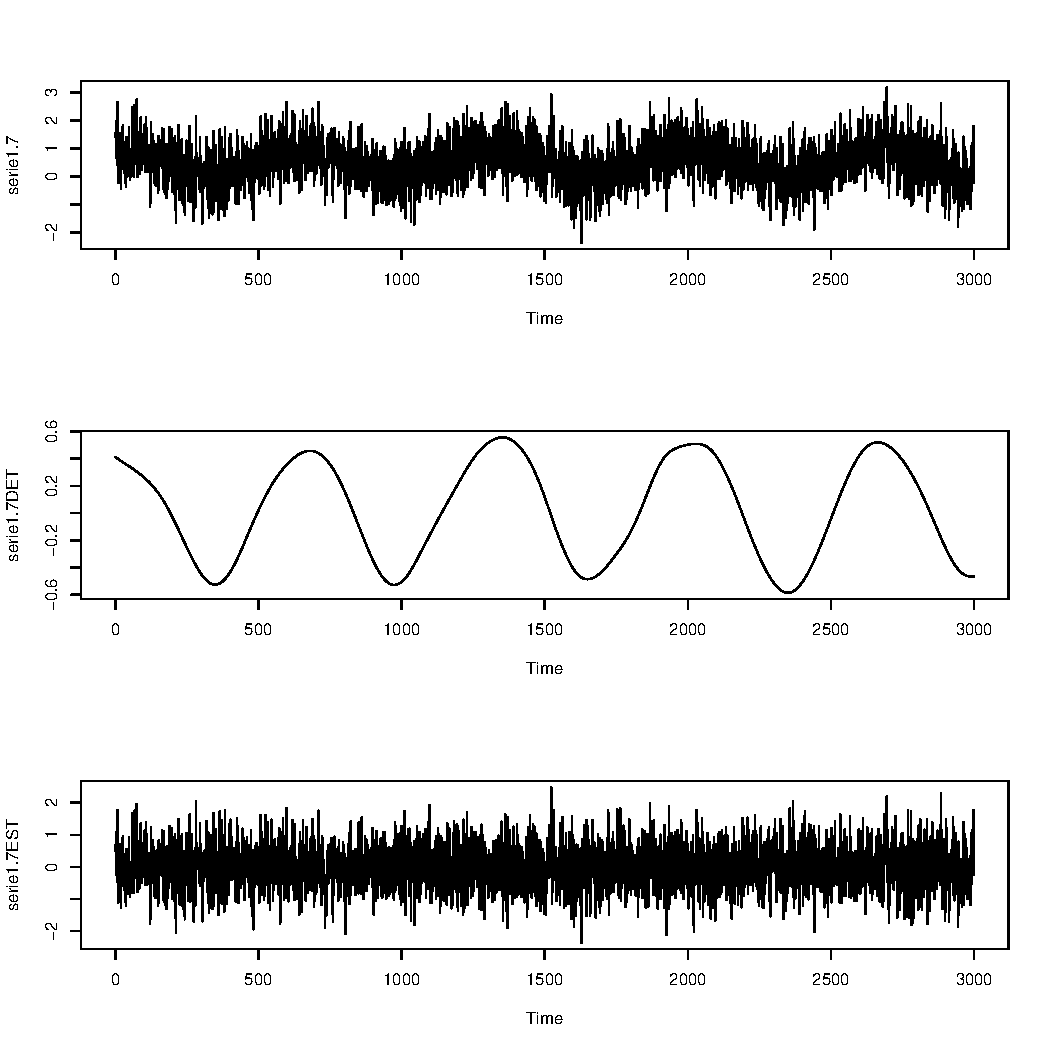
\includegraphics[scale=0.43]{serie1_7.pdf} \quad
  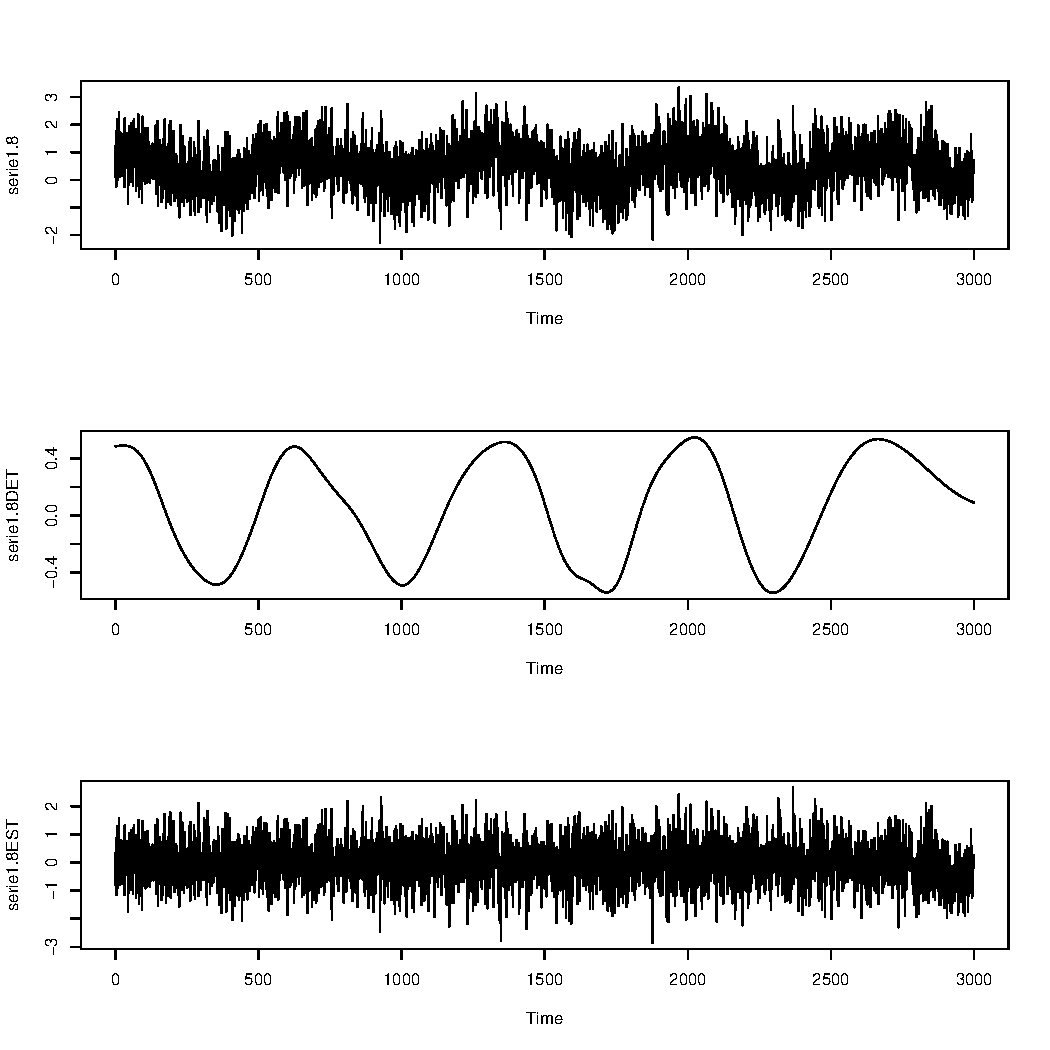
\includegraphics[scale=0.43]{serie1_8.pdf}
  \caption{Série 1.7 e Série 1.8}

\end{center}
\end{figure}

\graphicspath{{imagens/}}
\begin{figure}[H]
\begin{center}
  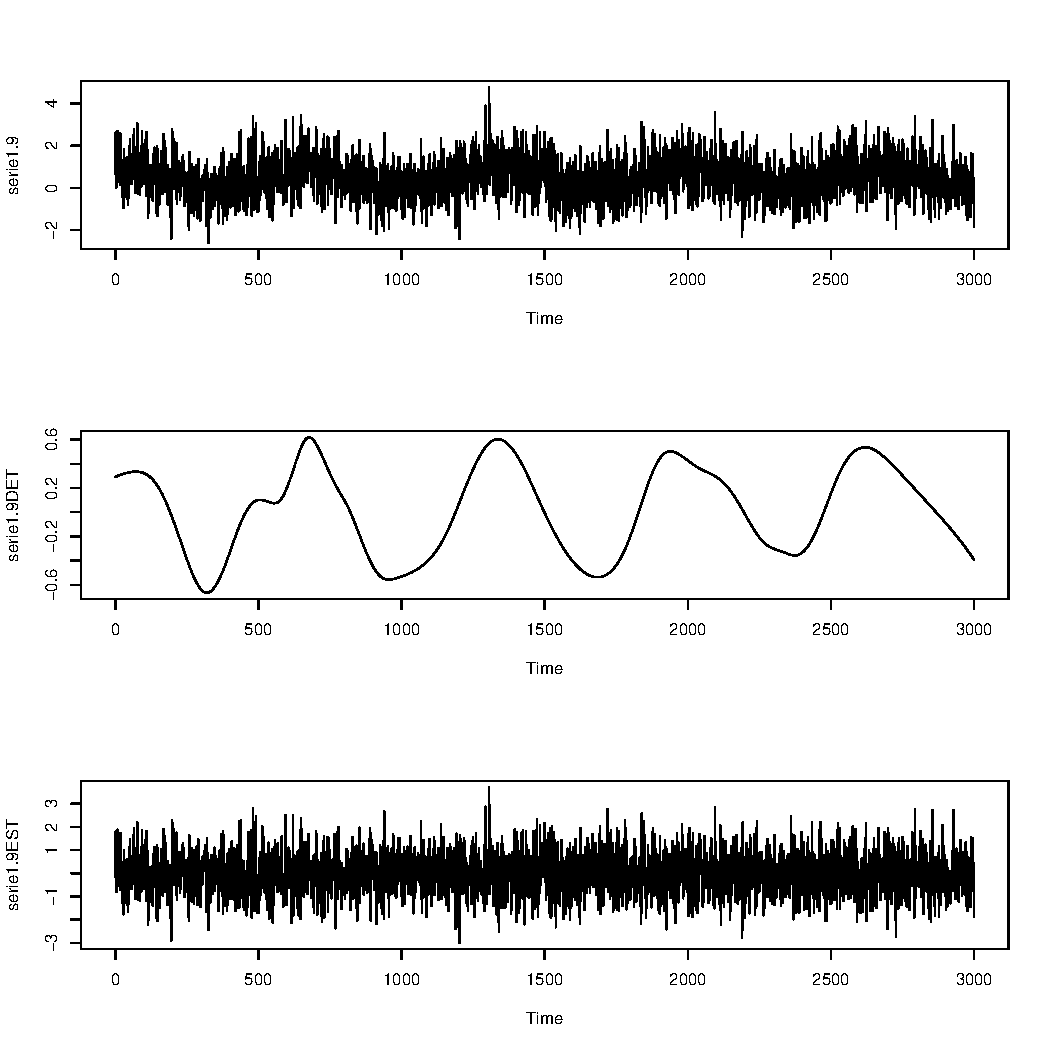
\includegraphics[scale=0.43]{serie1_9.pdf} \quad
  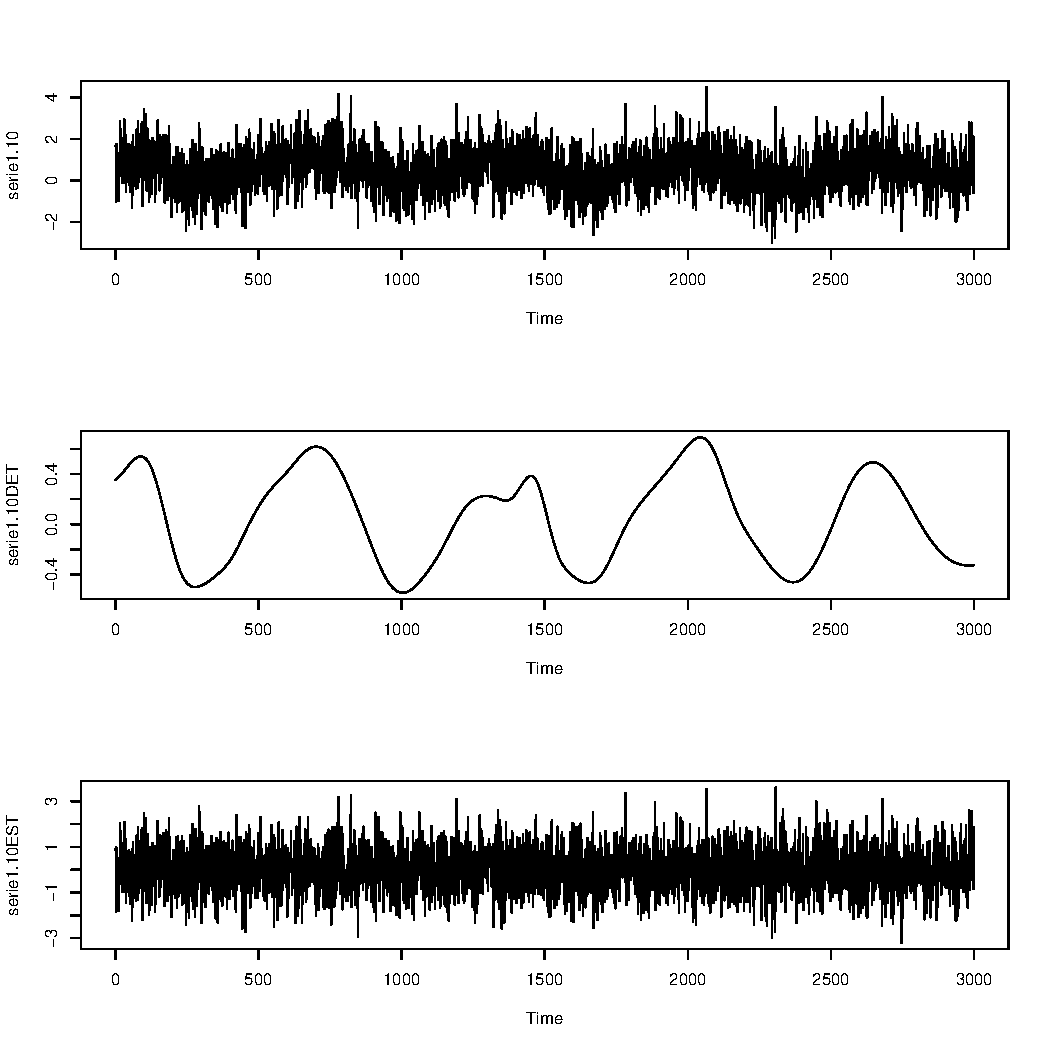
\includegraphics[scale=0.43]{serie1_10.pdf}
  \caption{Série 1.9 e Série 1.10}

\end{center}
\end{figure}

\section{Séries TIPO 2}
10 séries cossenoide com ruído ao longo da série e tendência.
\graphicspath{{imagens/}}
\begin{figure}[H]
\begin{center}
  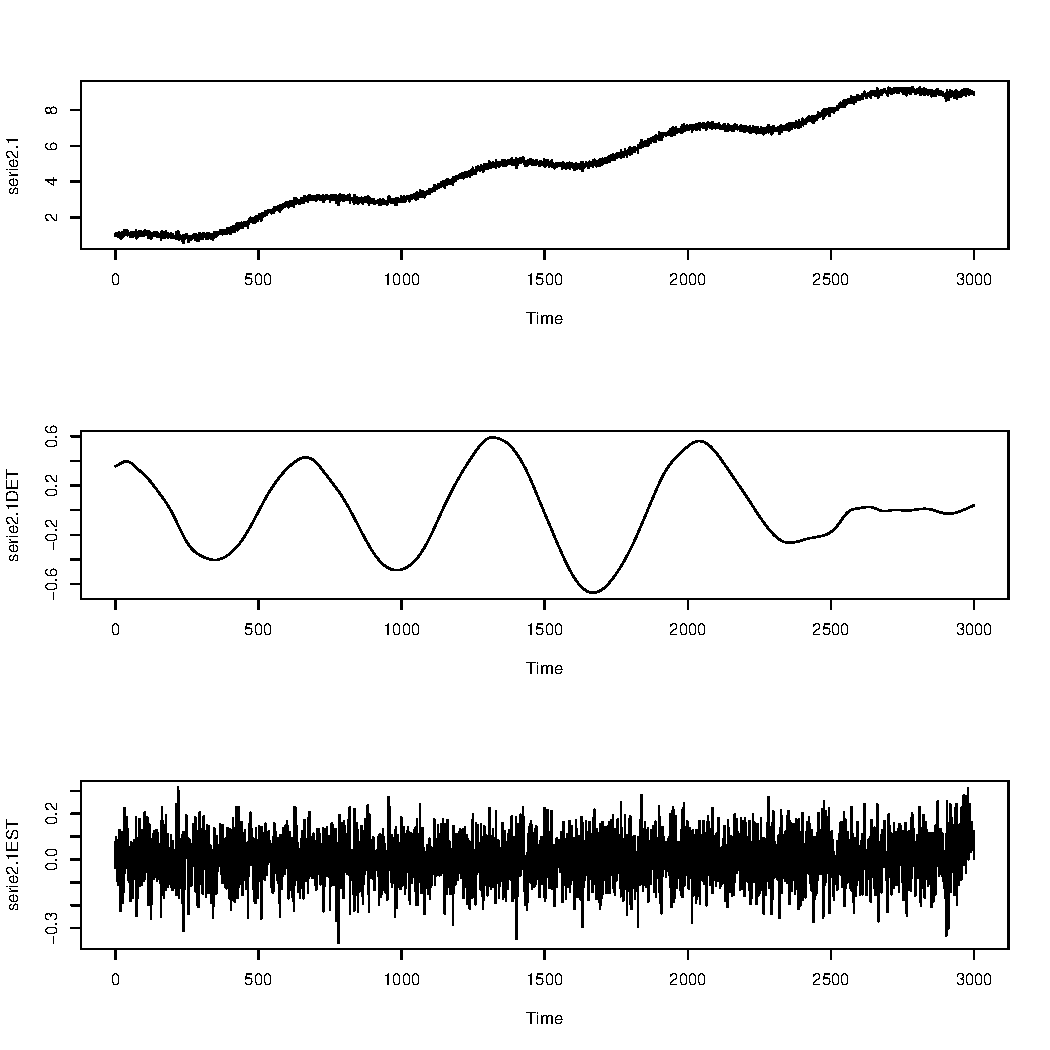
\includegraphics[scale=0.43]{serie2_1.pdf} \quad
  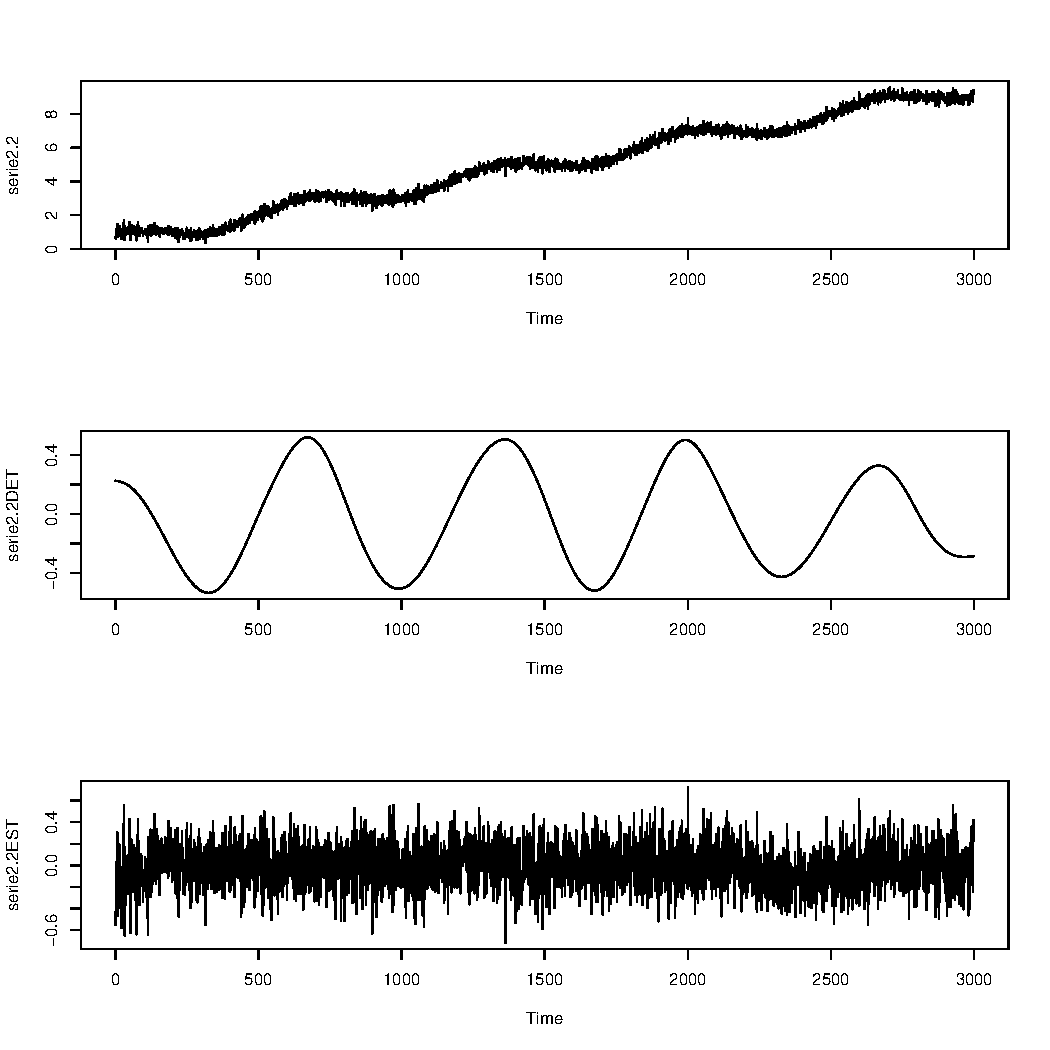
\includegraphics[scale=0.43]{serie2_2.pdf}
  \caption{Série 2.1 e Série 2.2}

\end{center}
\end{figure}

\graphicspath{{imagens/}}
\begin{figure}[H]
\begin{center}
  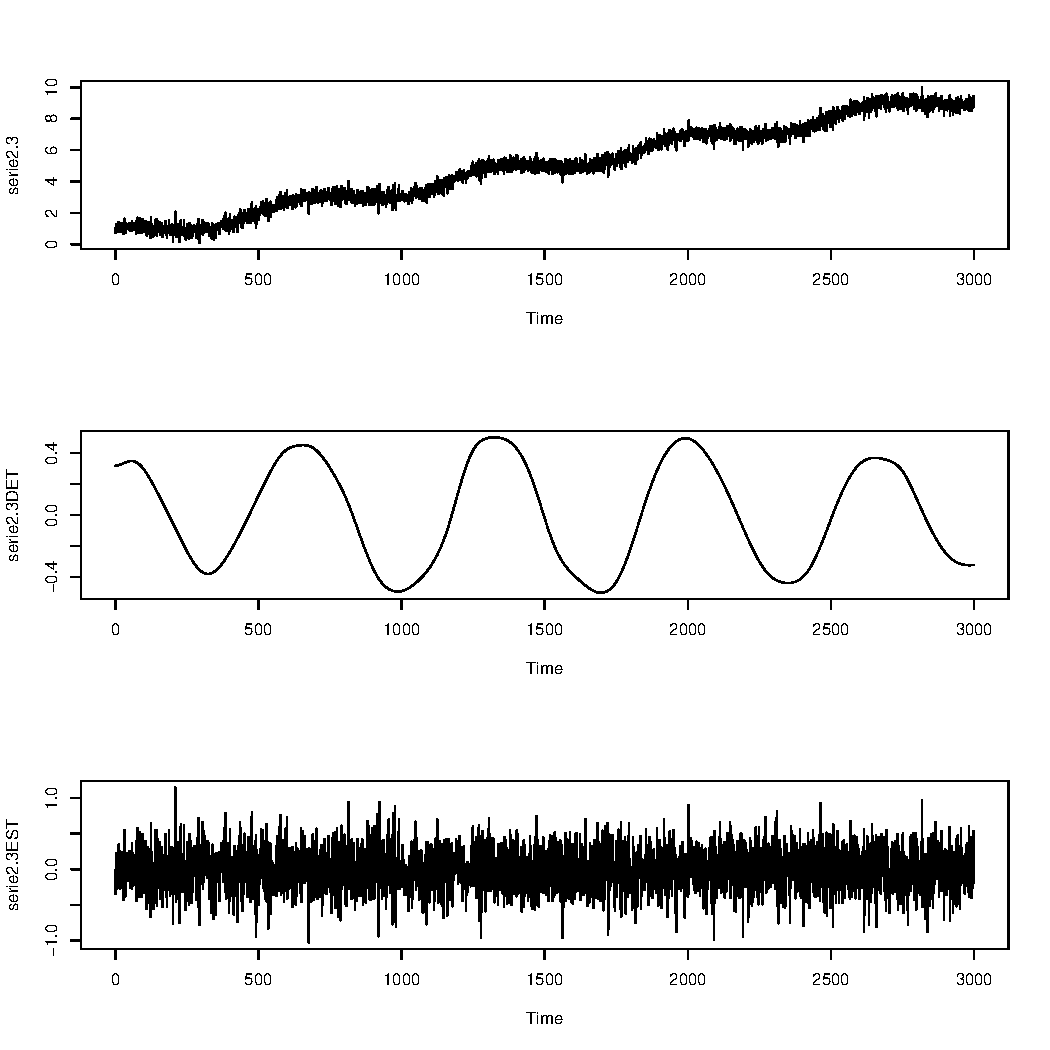
\includegraphics[scale=0.43]{serie2_3.pdf} \quad
  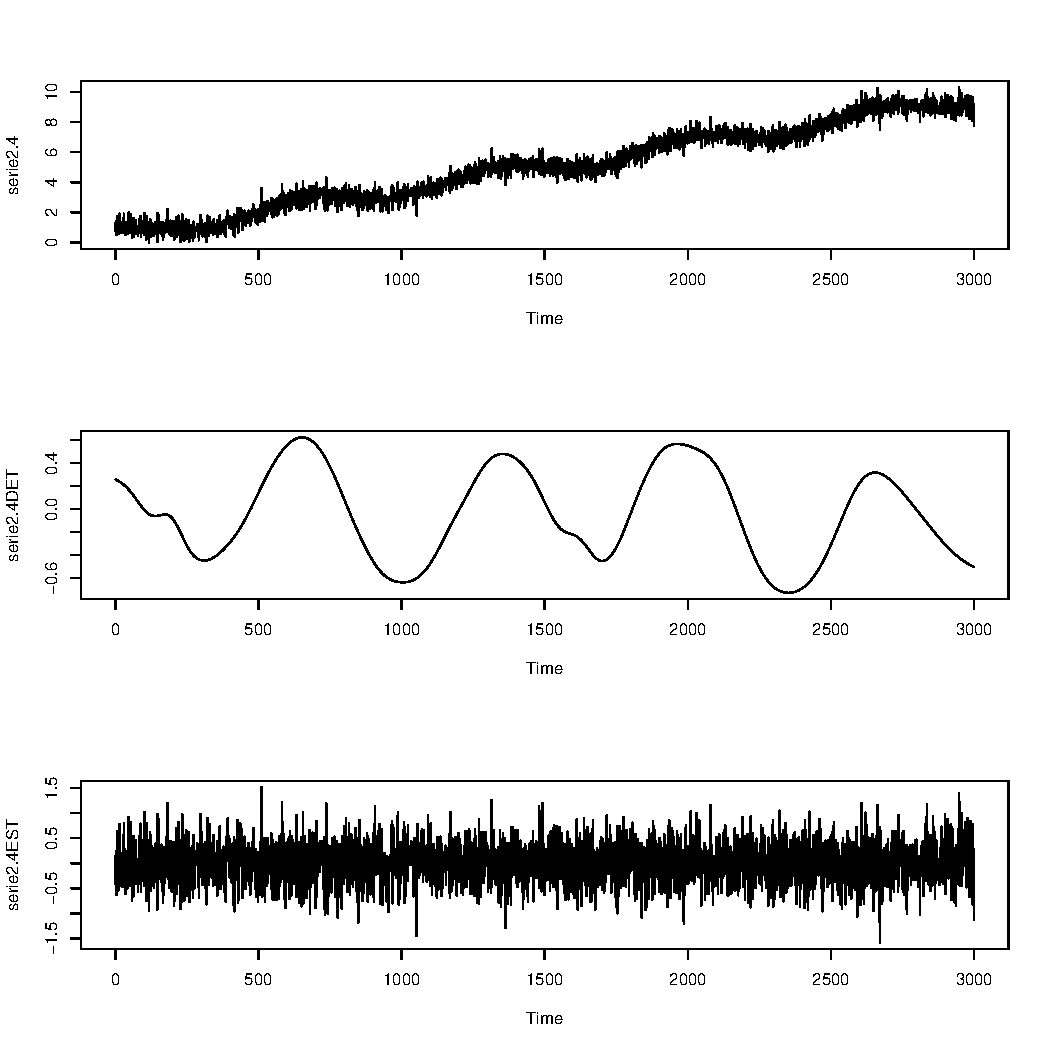
\includegraphics[scale=0.43]{serie2_4.pdf}
  \caption{Série 2.3 e Série 2.4}

\end{center}
\end{figure}

\graphicspath{{imagens/}}
\begin{figure}[H]
\begin{center}
  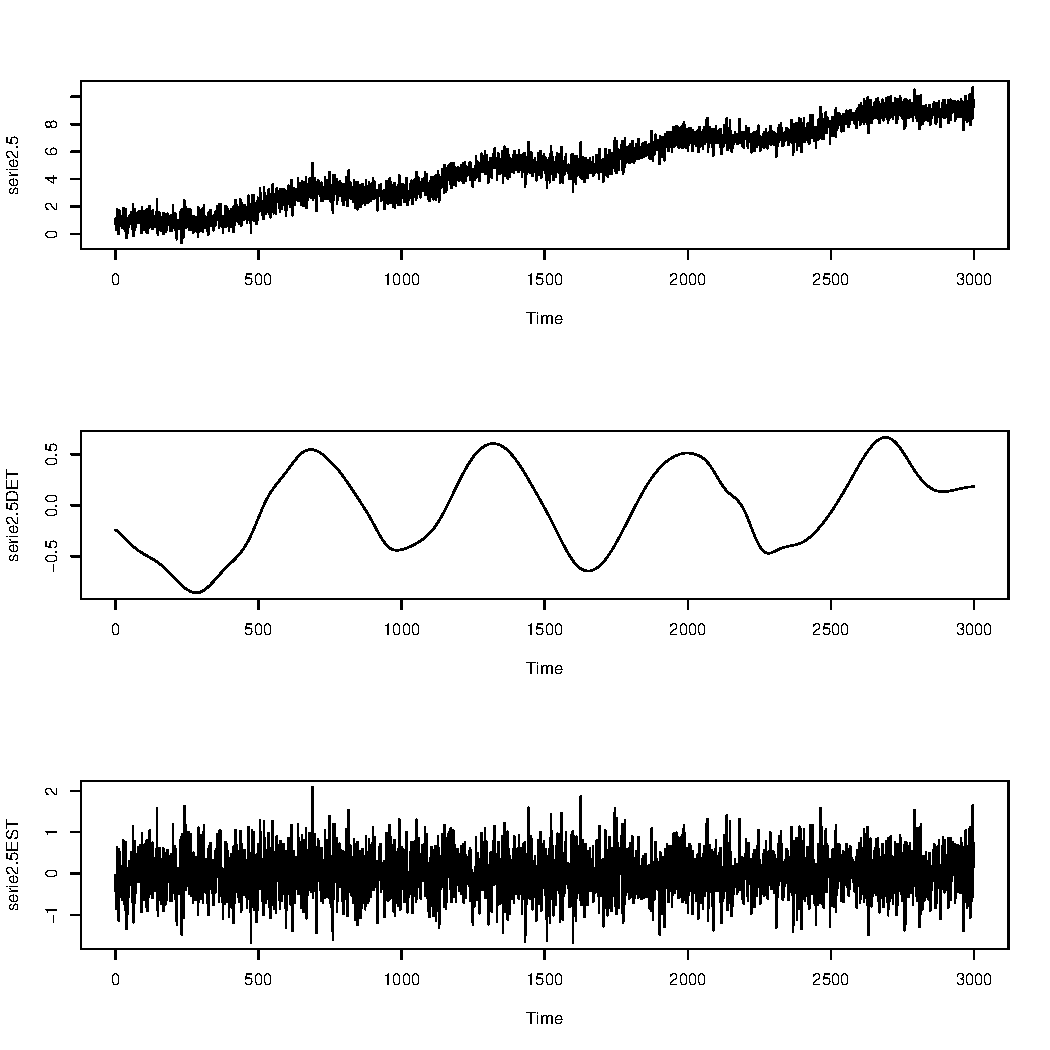
\includegraphics[scale=0.43]{serie2_5.pdf} \quad
  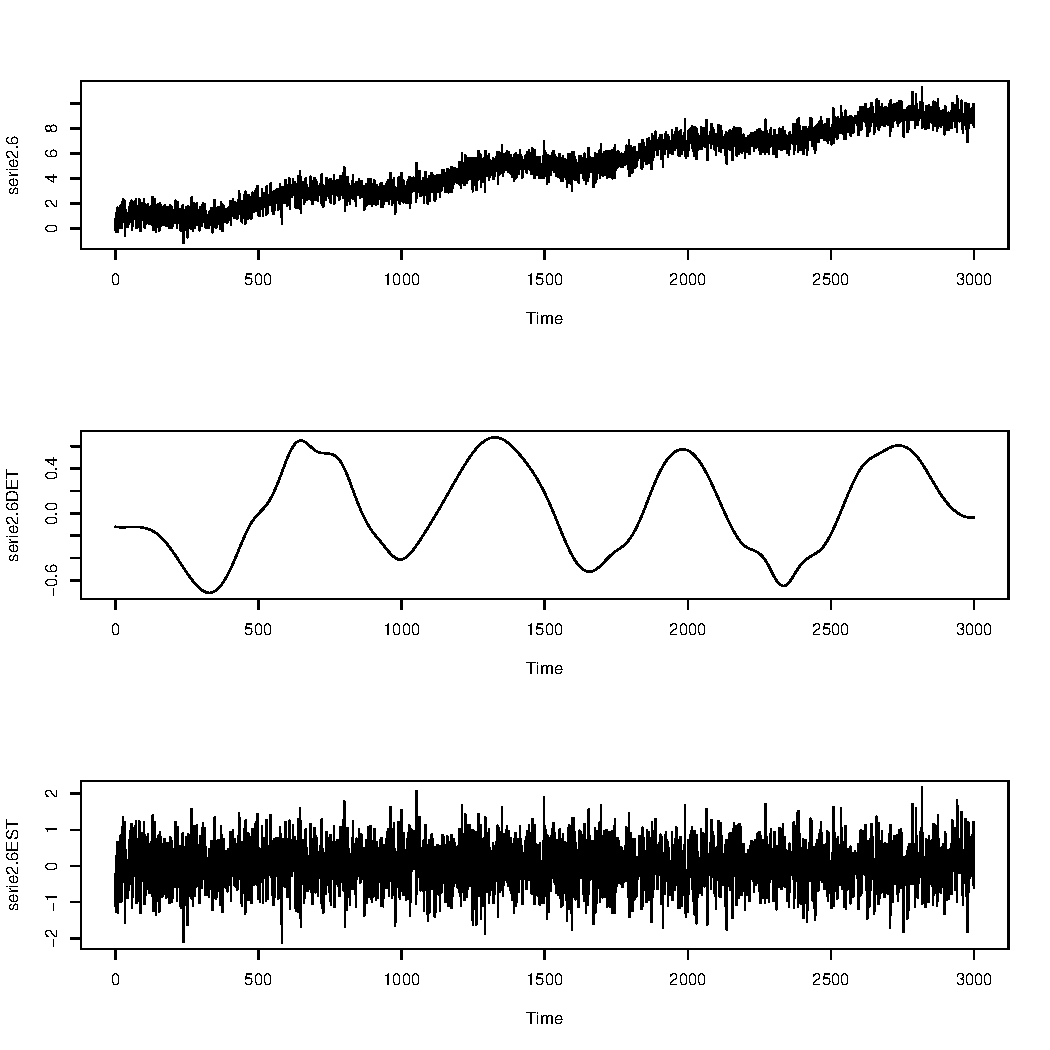
\includegraphics[scale=0.43]{serie2_6.pdf}
  \caption{Série 2.5 e Série 2.6}

\end{center}
\end{figure}

\graphicspath{{imagens/}}
\begin{figure}[H]
\begin{center}
  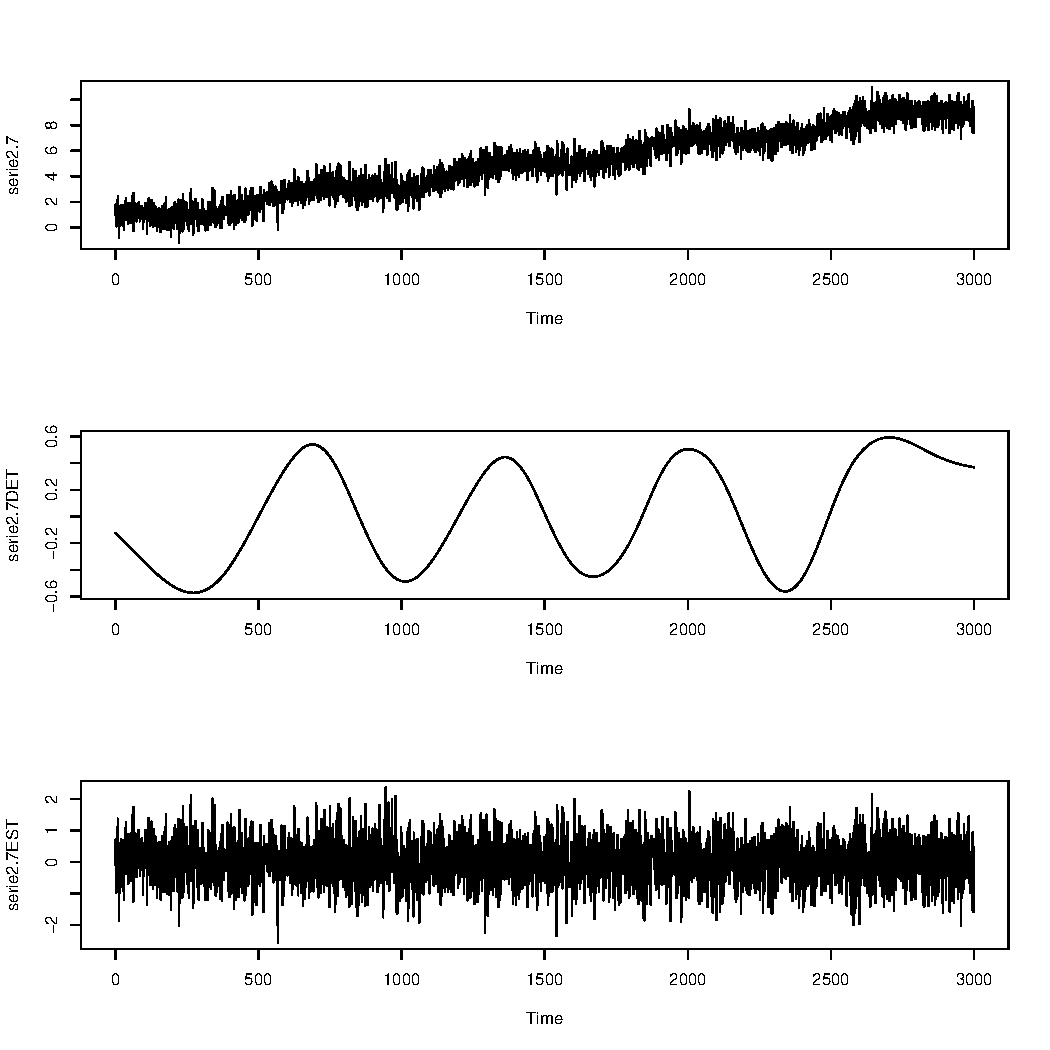
\includegraphics[scale=0.43]{serie2_7.pdf} \quad
  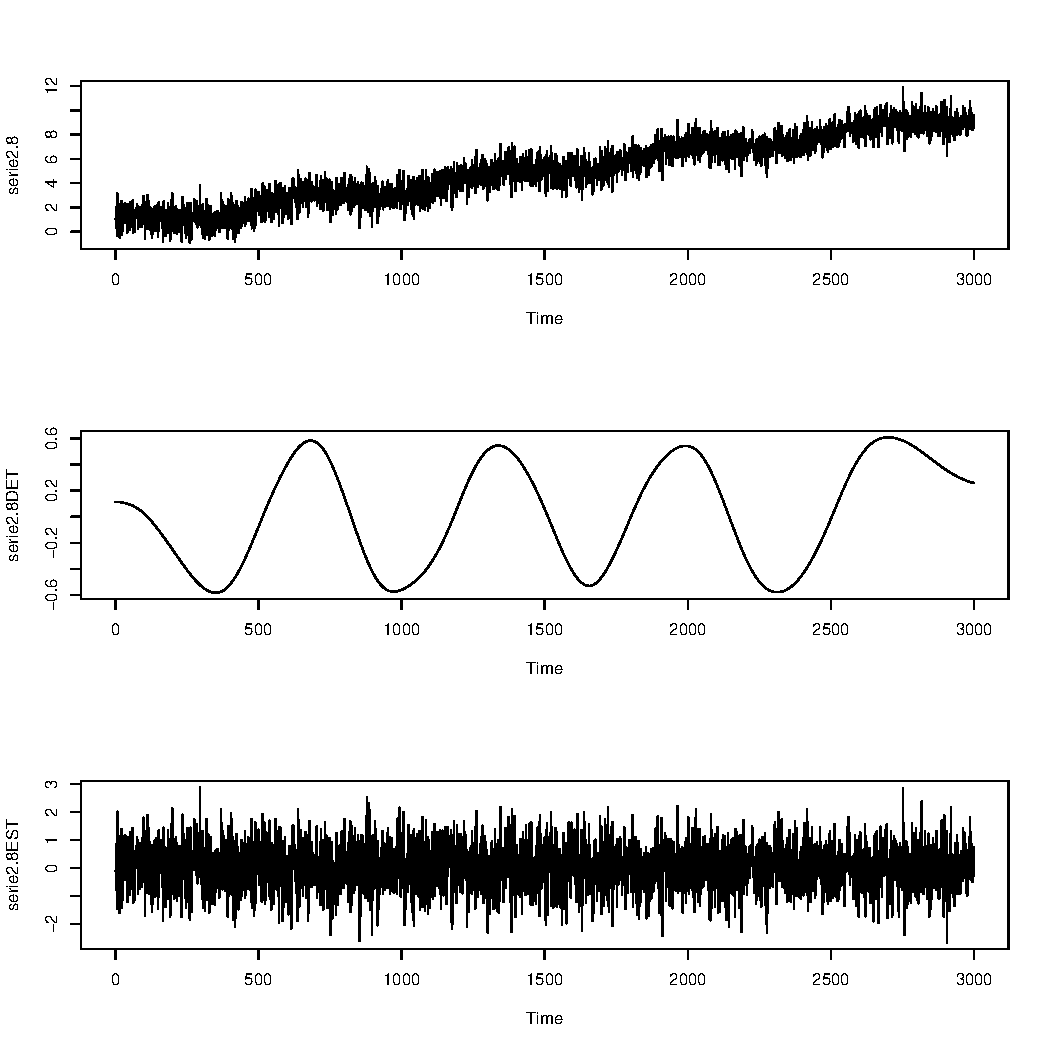
\includegraphics[scale=0.43]{serie2_8.pdf}
  \caption{Série 2.7 e Série 2.8}

\end{center}
\end{figure}

\graphicspath{{imagens/}}
\begin{figure}[H]
\begin{center}
  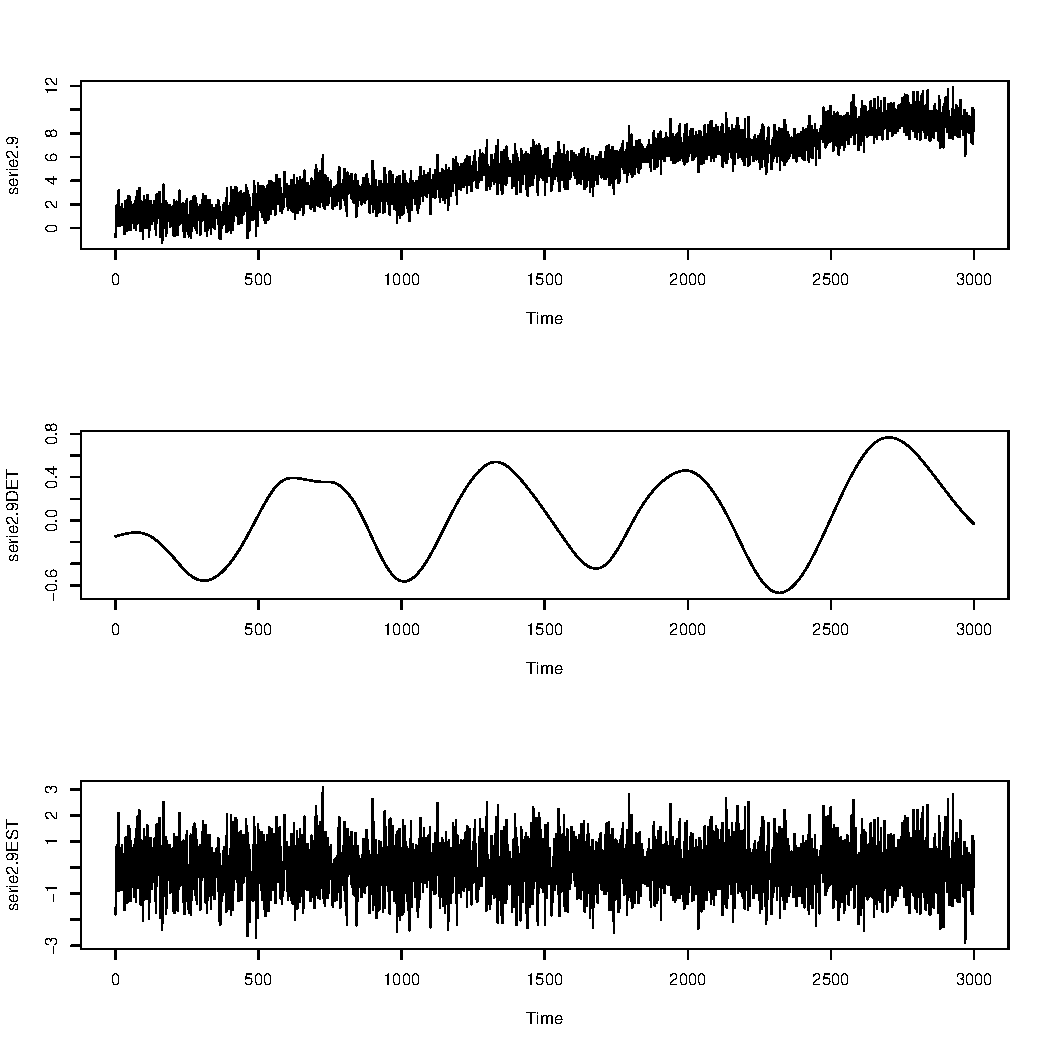
\includegraphics[scale=0.43]{serie2_9.pdf} \quad
  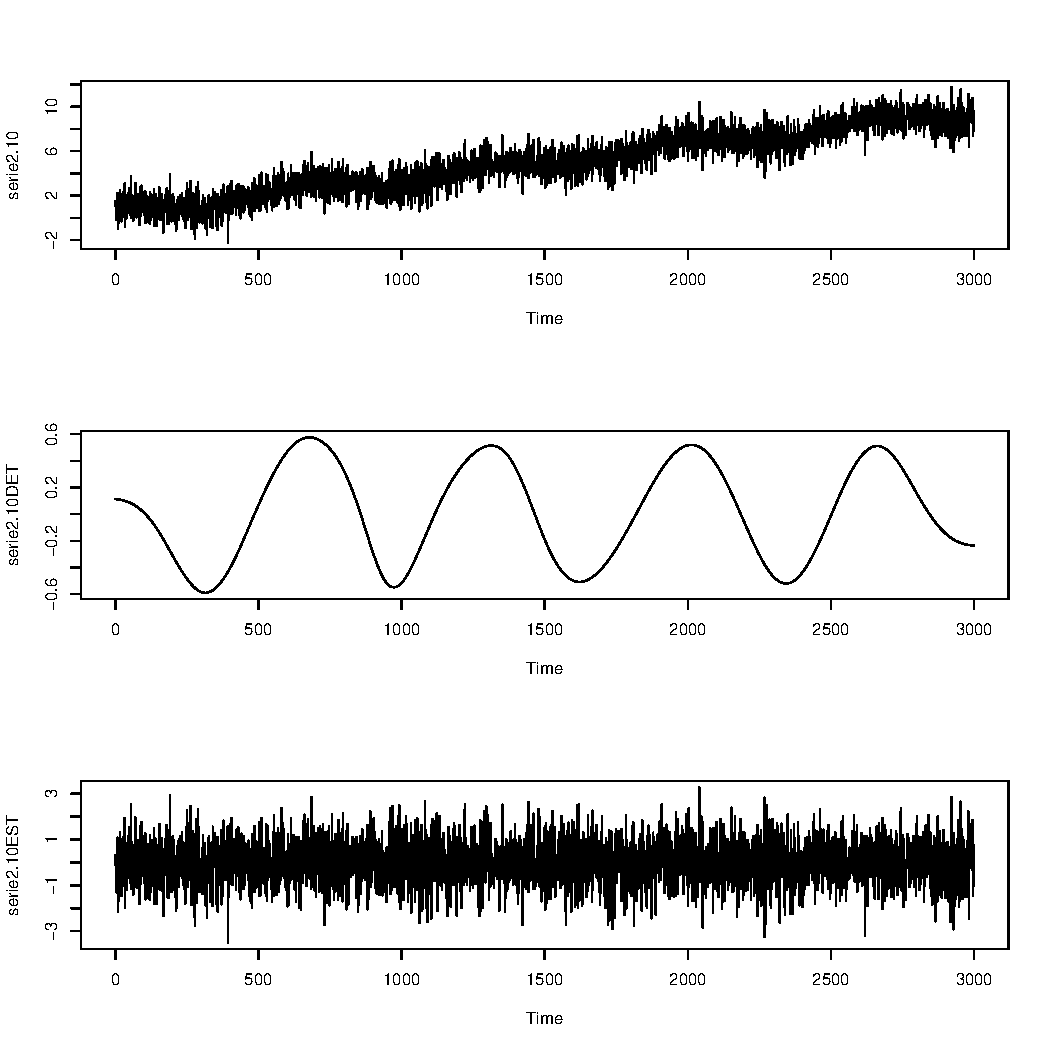
\includegraphics[scale=0.43]{serie2_10.pdf}
  \caption{Série 2.9 e Série 2.10}

\end{center}
\end{figure}

\section{Séries TIPO 3}
10 séries senoide com ruído ao longo da série.
\graphicspath{{imagens/}}
\begin{figure}[H]
\begin{center}
  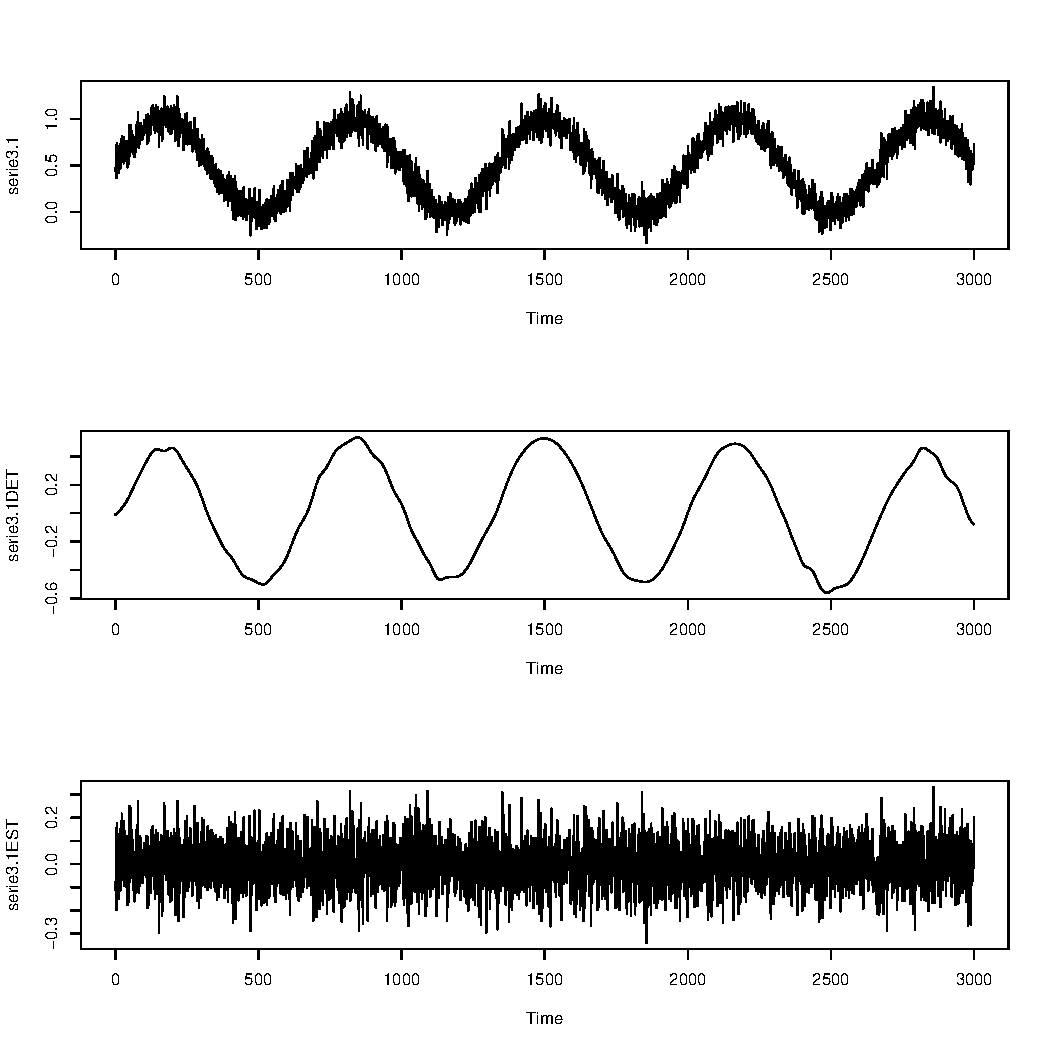
\includegraphics[scale=0.43]{serie3_1.pdf} \quad
  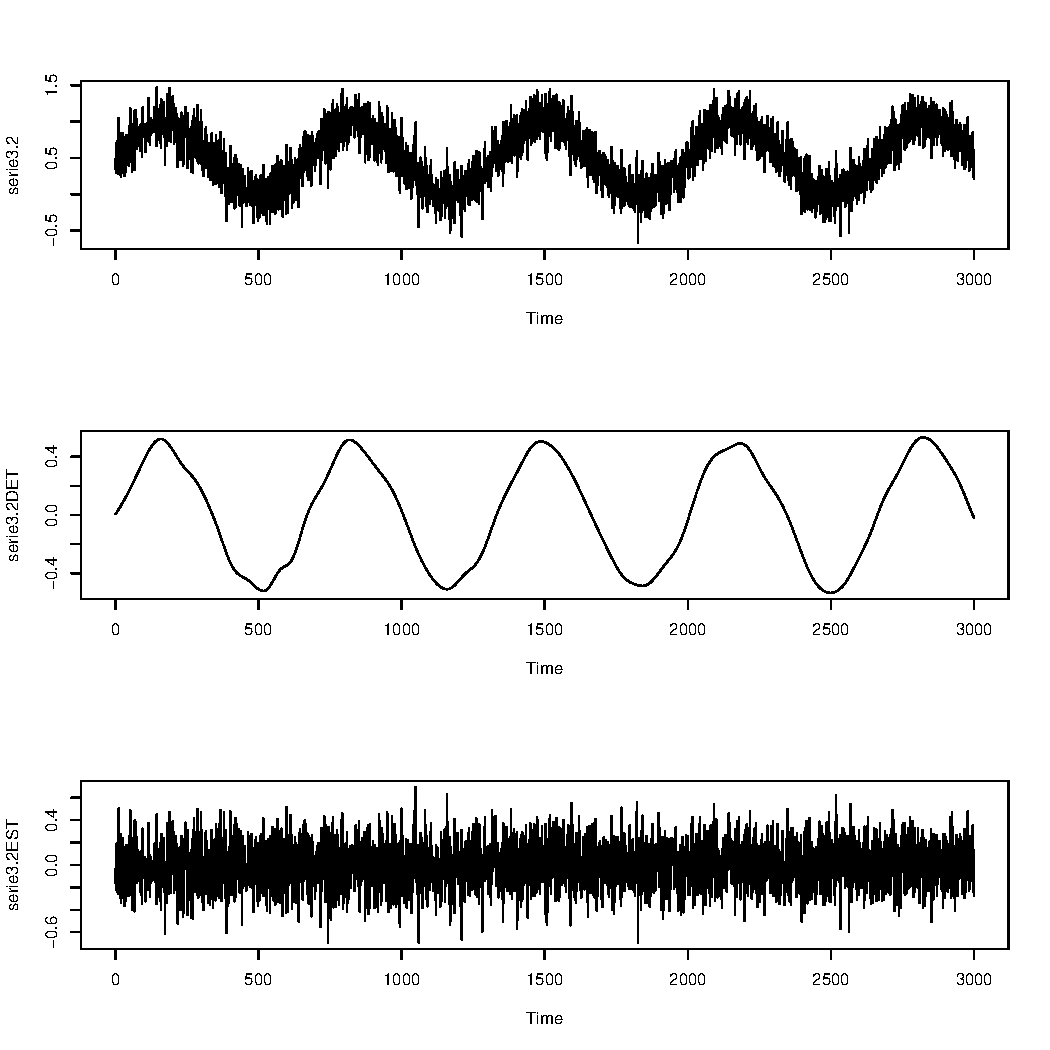
\includegraphics[scale=0.43]{serie3_2.pdf}
  \caption{Série 3.1 e Série 3.2}

\end{center}
\end{figure}

\graphicspath{{imagens/}}
\begin{figure}[H]
\begin{center}
  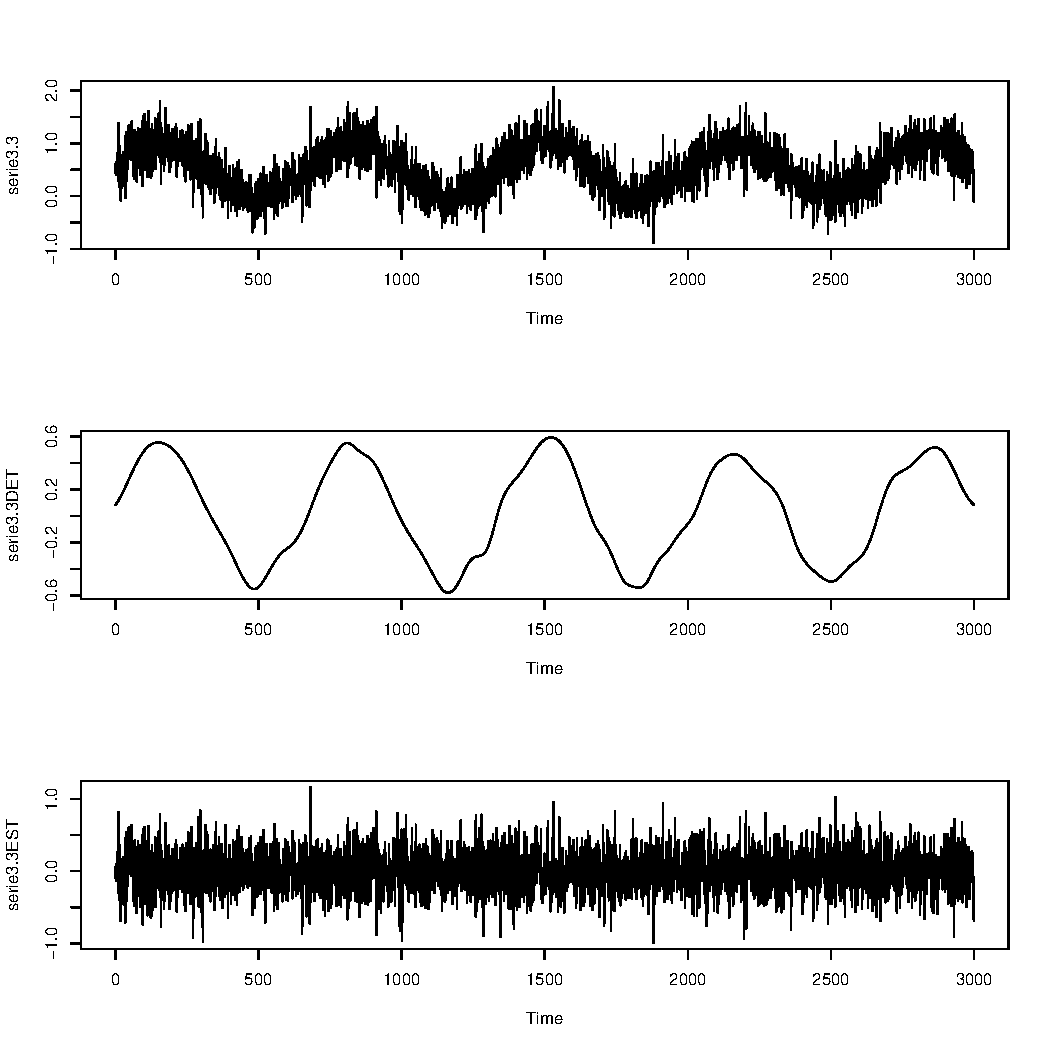
\includegraphics[scale=0.43]{serie3_3.pdf} \quad
  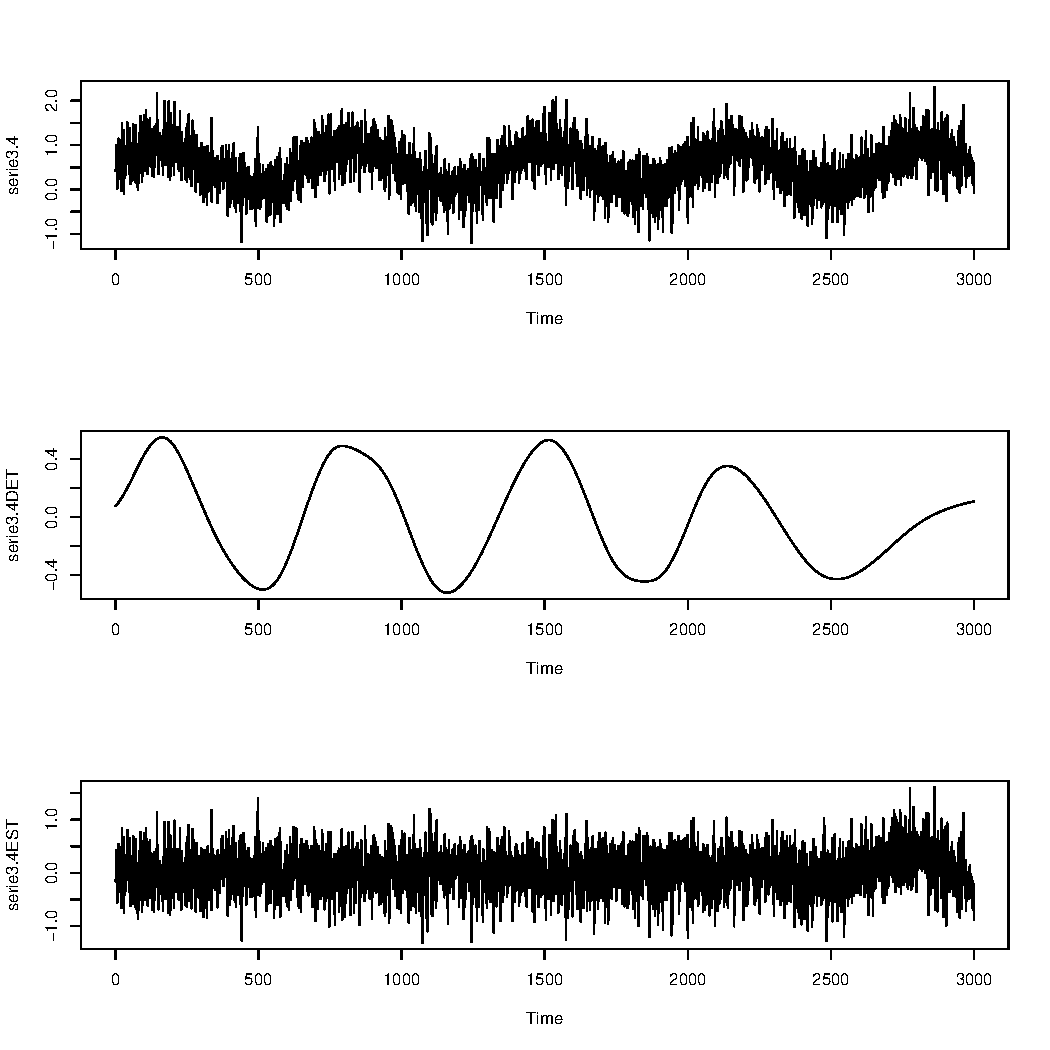
\includegraphics[scale=0.43]{serie3_4.pdf}
  \caption{Série 3.3 e Série 3.4}

\end{center}
\end{figure}

\graphicspath{{imagens/}}
\begin{figure}[H]
\begin{center}
  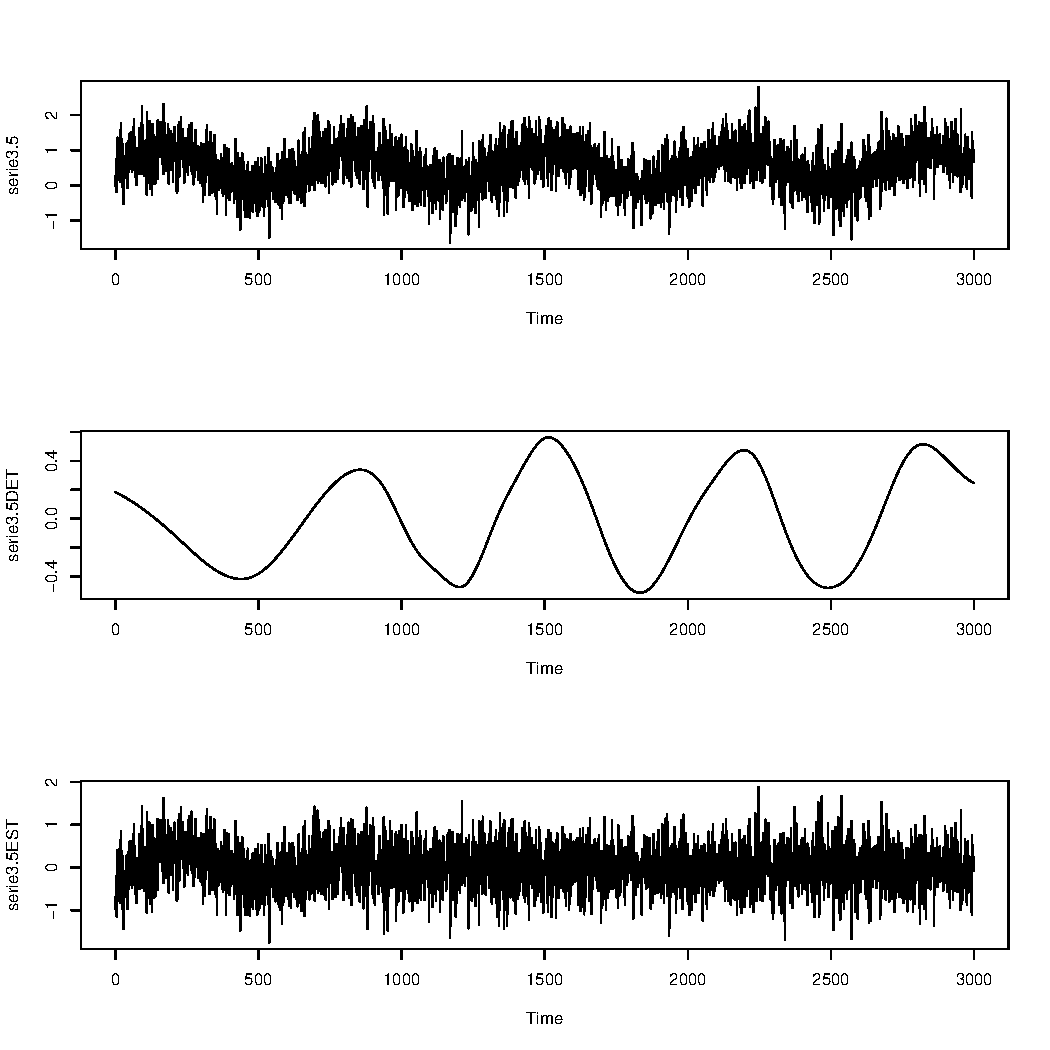
\includegraphics[scale=0.43]{serie3_5.pdf} \quad
  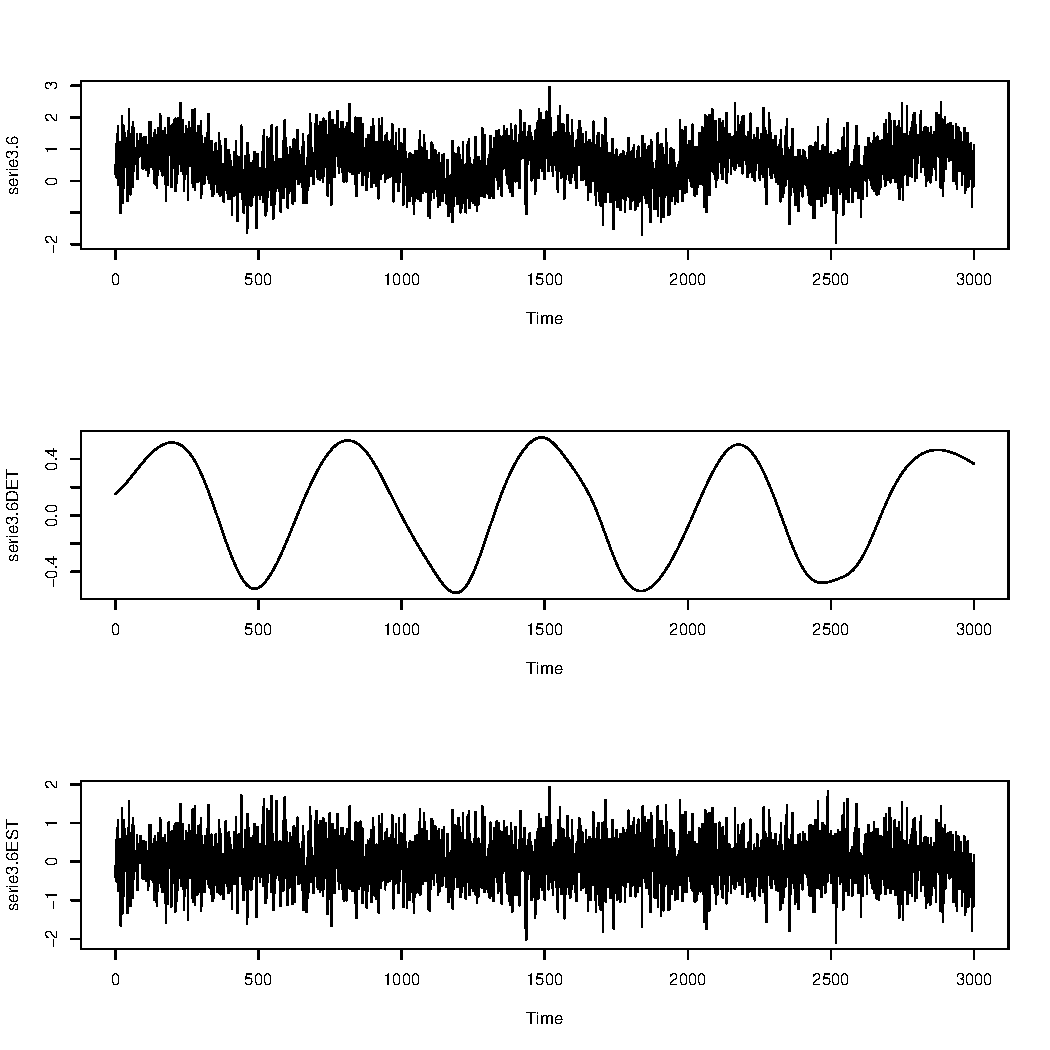
\includegraphics[scale=0.43]{serie3_6.pdf}
  \caption{Série 3.5 e Série 3.6}

\end{center}
\end{figure}

\graphicspath{{imagens/}}
\begin{figure}[H]
\begin{center}
  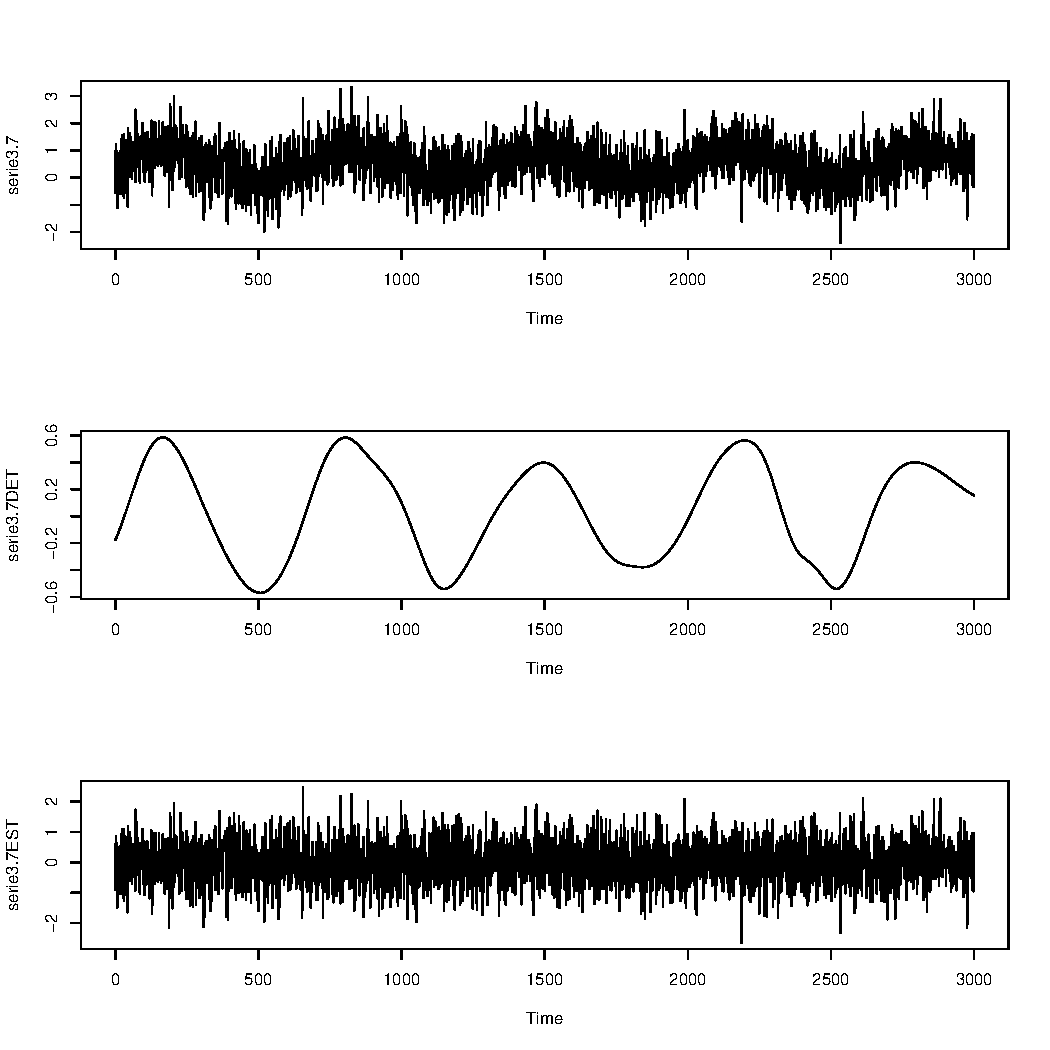
\includegraphics[scale=0.43]{serie3_7.pdf} \quad
  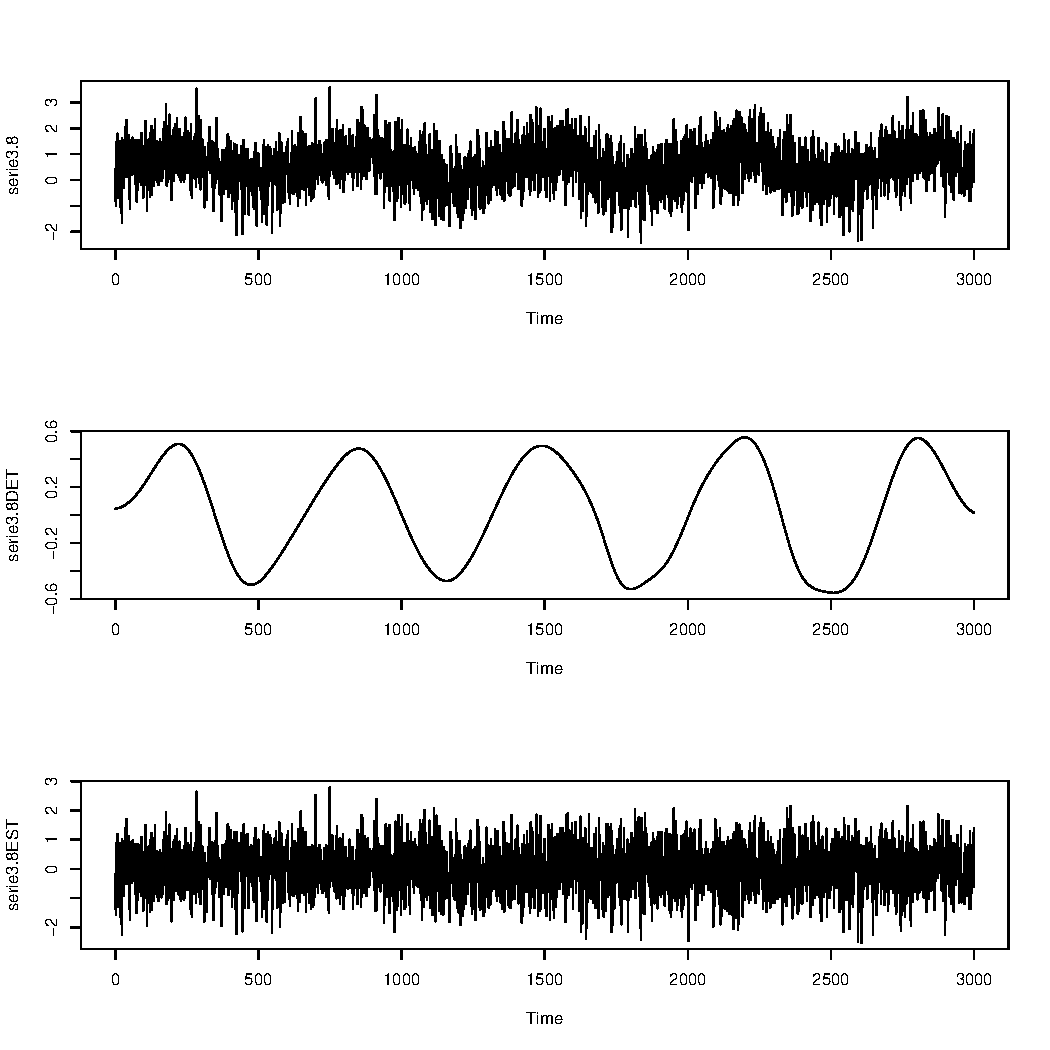
\includegraphics[scale=0.43]{serie3_8.pdf}
  \caption{Série 3.7 e Série 3.8}

\end{center}
\end{figure}

\graphicspath{{imagens/}}
\begin{figure}[H]
\begin{center}
  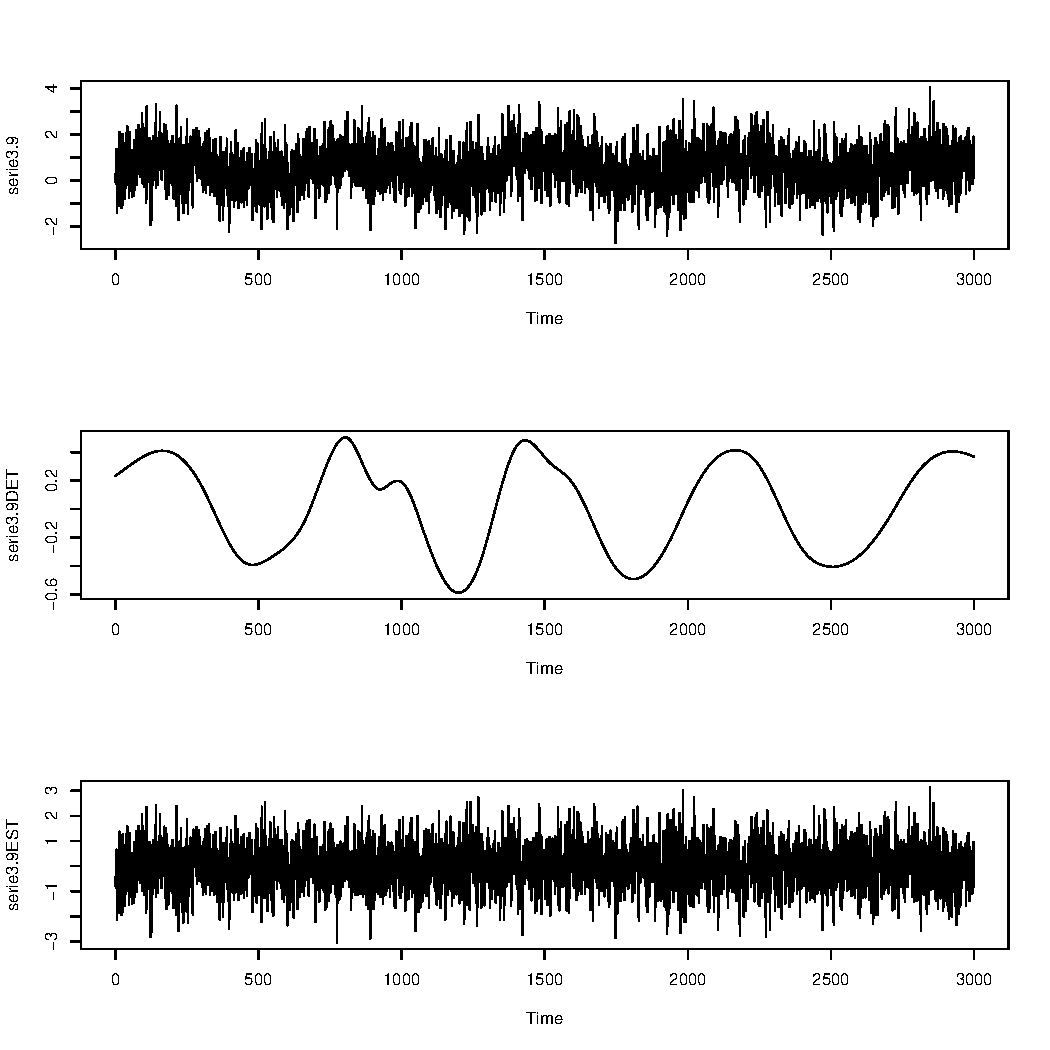
\includegraphics[scale=0.43]{serie3_9.pdf} \quad
  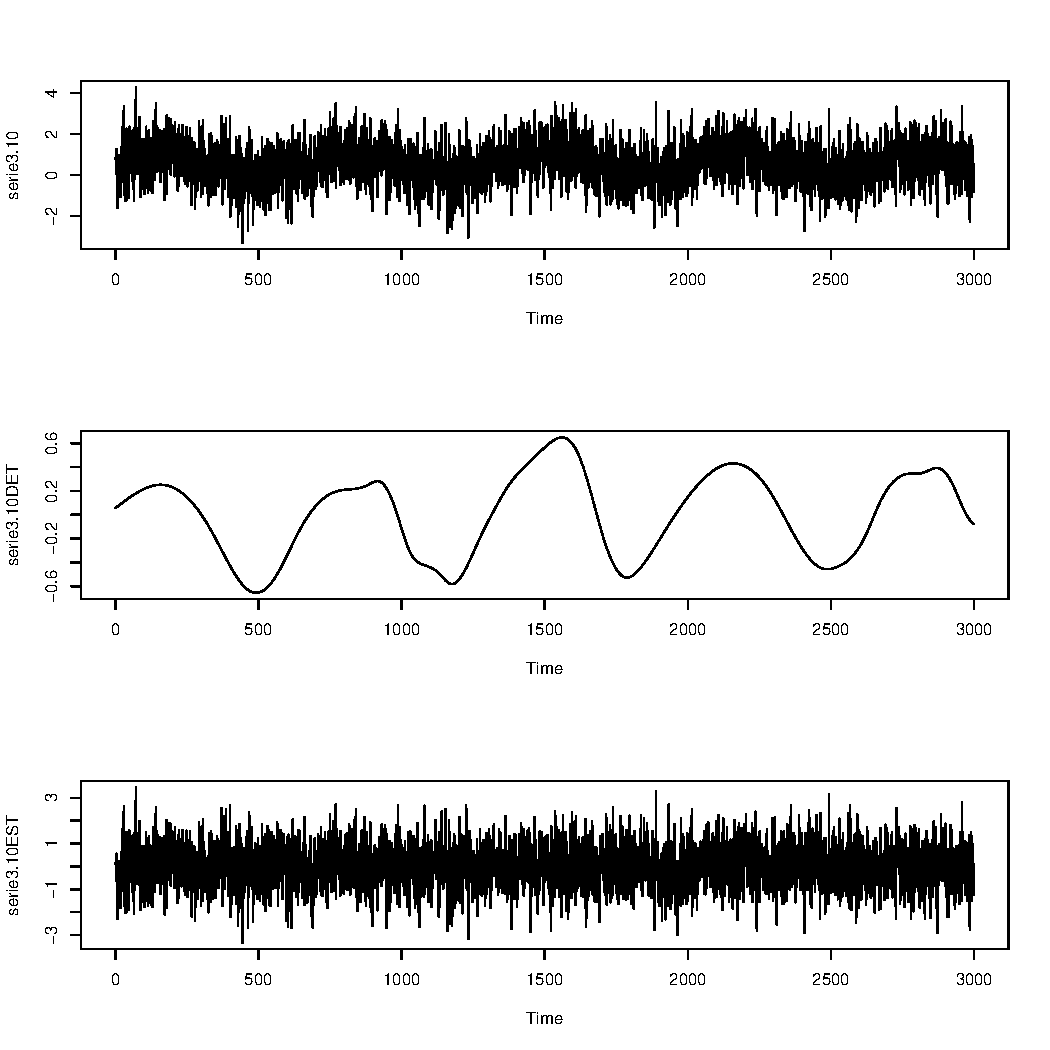
\includegraphics[scale=0.43]{serie3_10.pdf}
  \caption{Série 3.9 e Série 3.10}

\end{center}
\end{figure}

\section{Séries TIPO 4}
10 séries senoide com ruído ao longo da série e tendência.
\graphicspath{{imagens/}}
\begin{figure}[H]
\begin{center}
  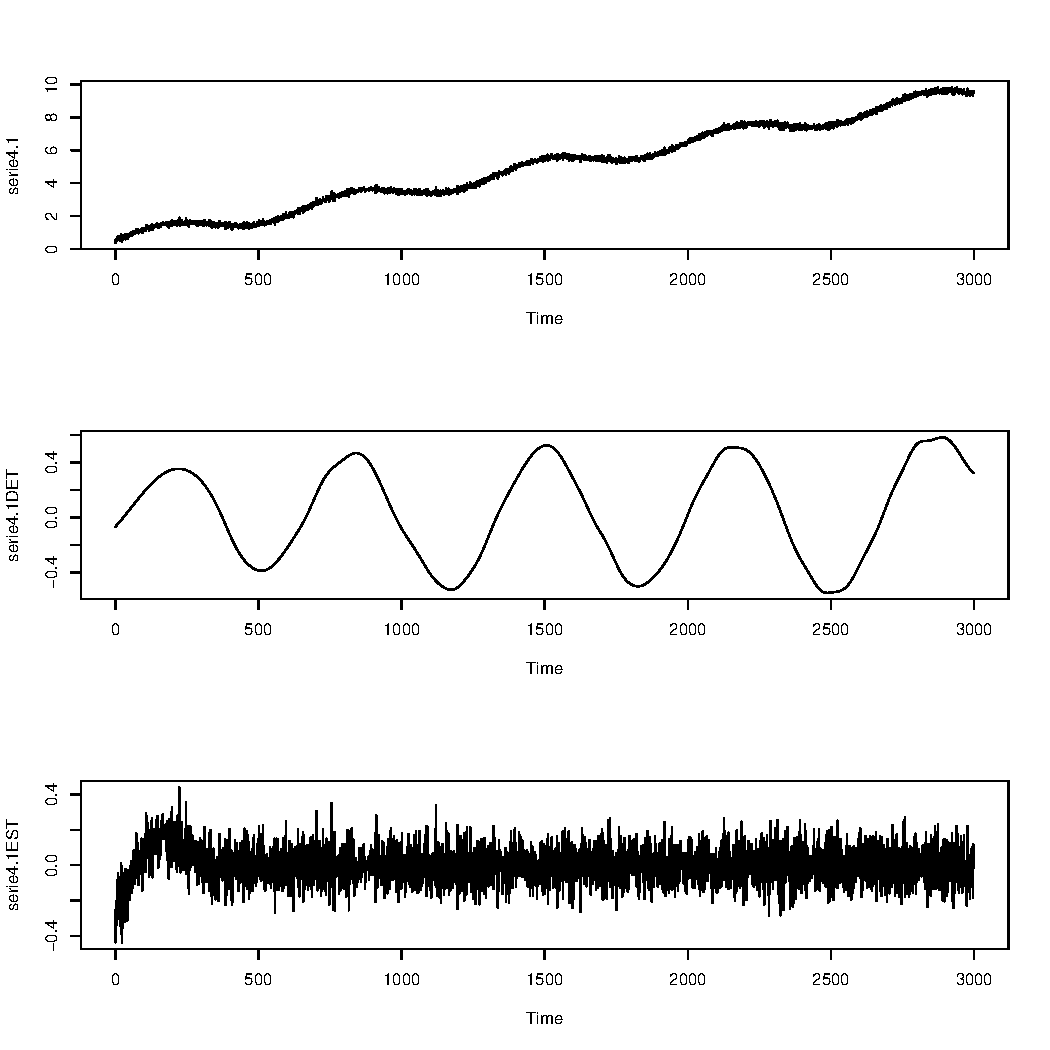
\includegraphics[scale=0.43]{serie4_1.pdf} \quad
  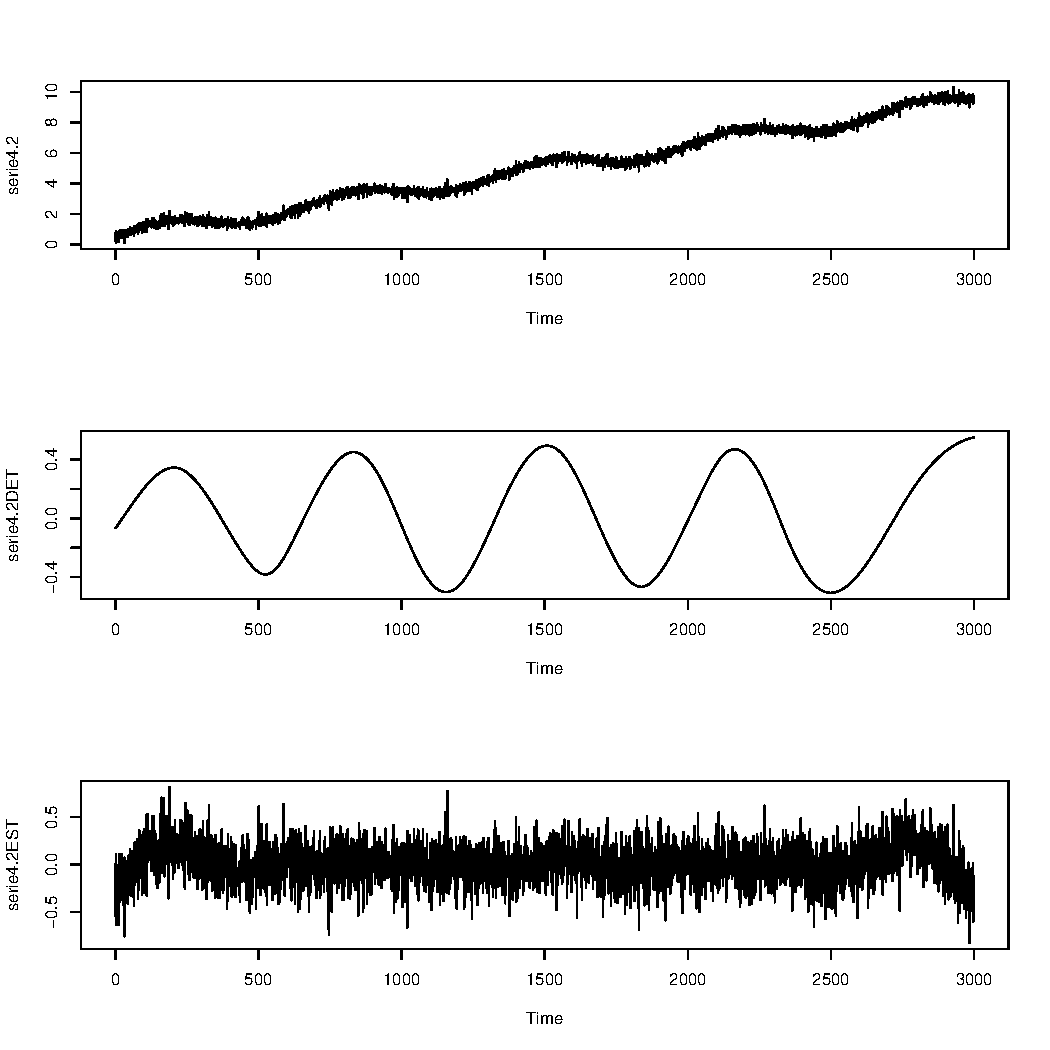
\includegraphics[scale=0.43]{serie4_2.pdf}
  \caption{Série 4.1 e Série 4.2}
\end{center}
\end{figure}

\graphicspath{{imagens/}}
\begin{figure}[H]
\begin{center}
  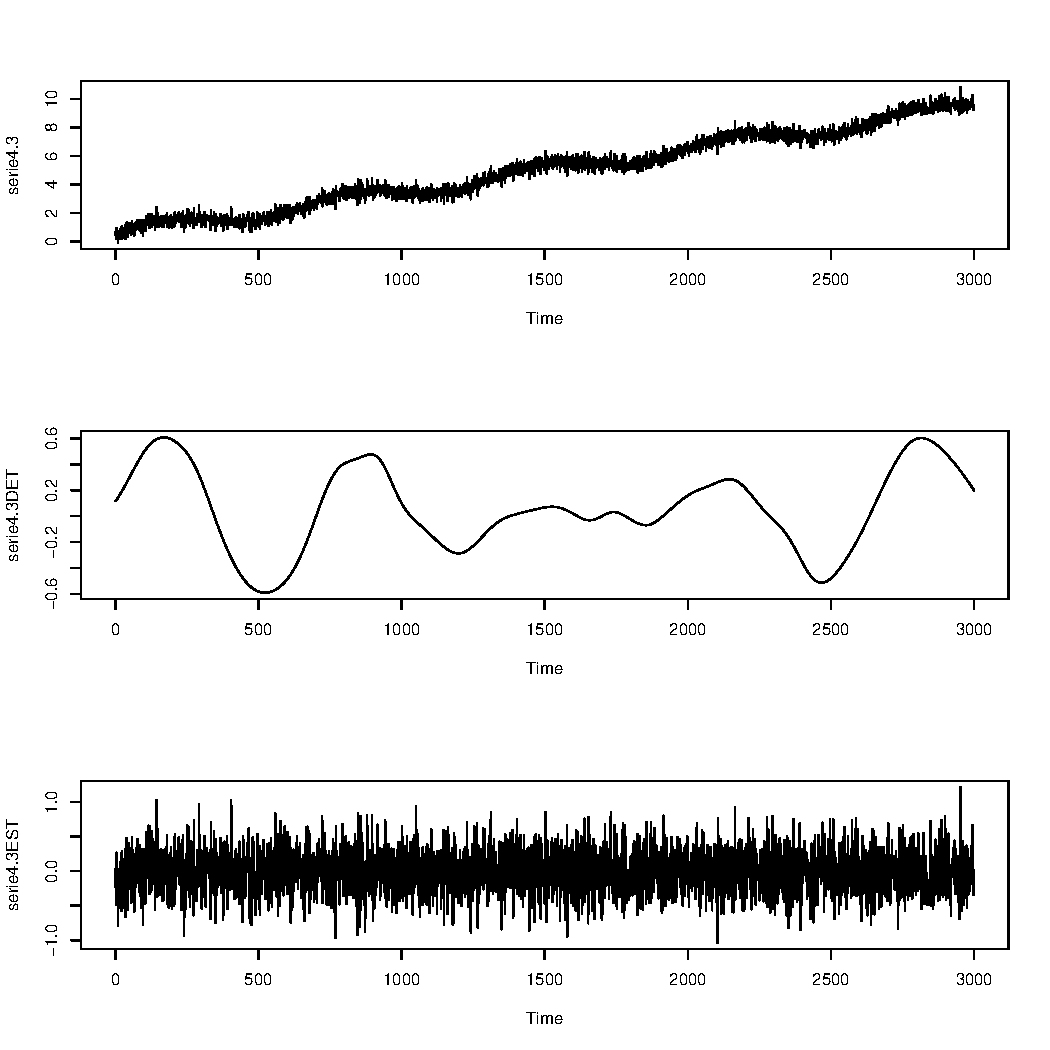
\includegraphics[scale=0.43]{serie4_3.pdf} \quad
 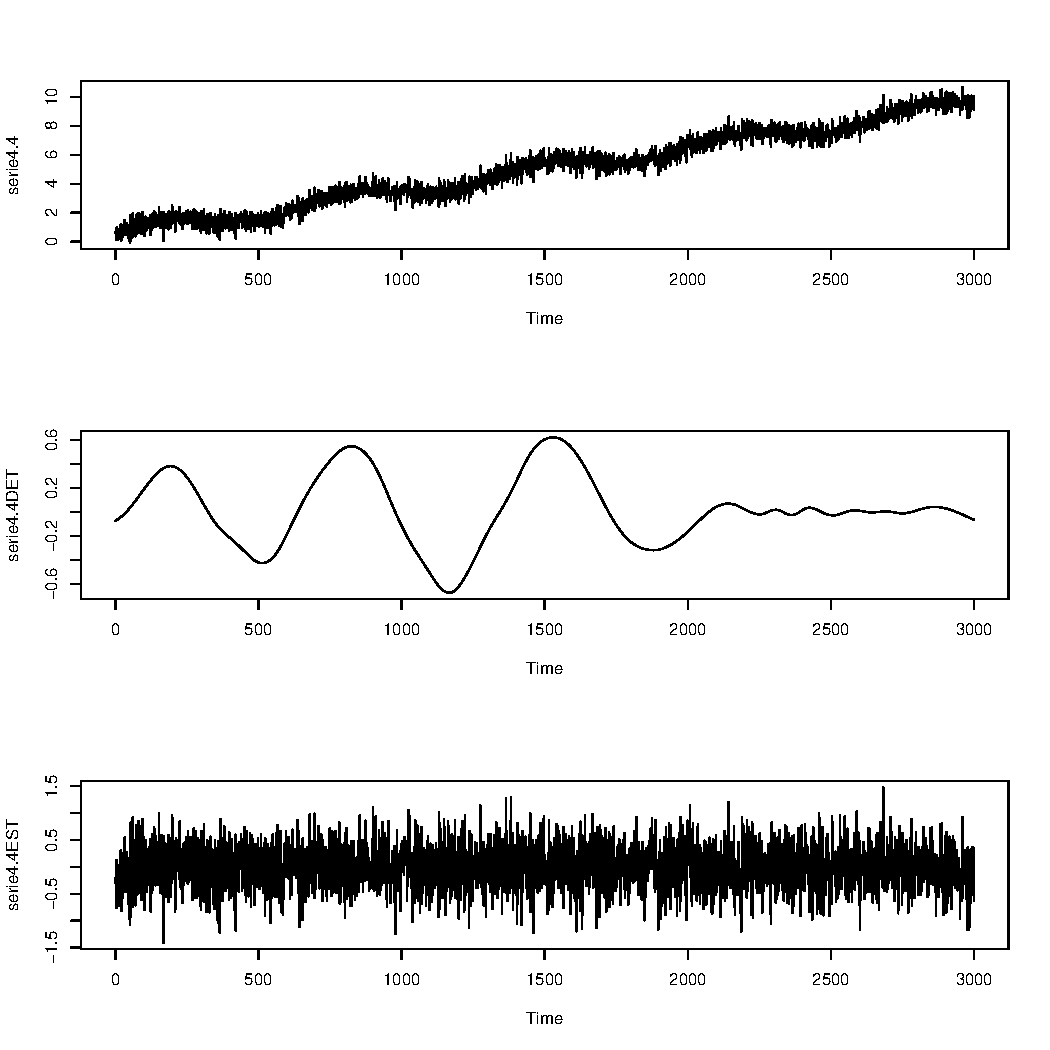
\includegraphics[scale=0.43]{serie4_4.pdf}
 \caption{Série 4.3 e Série 4.4}

\end{center}
\end{figure}

\graphicspath{{imagens/}}
\begin{figure}[H]
\begin{center}
  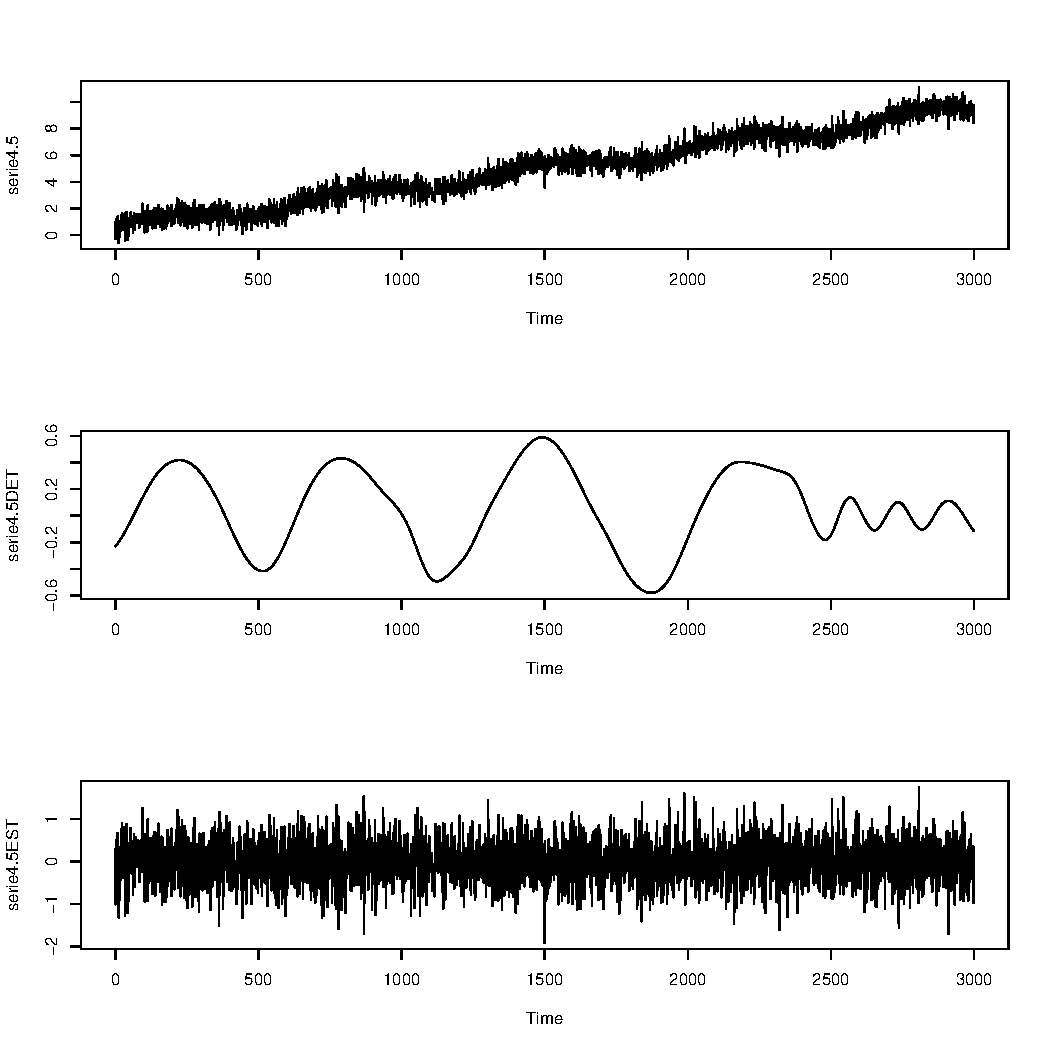
\includegraphics[scale=0.43]{serie4_5.pdf} \quad
  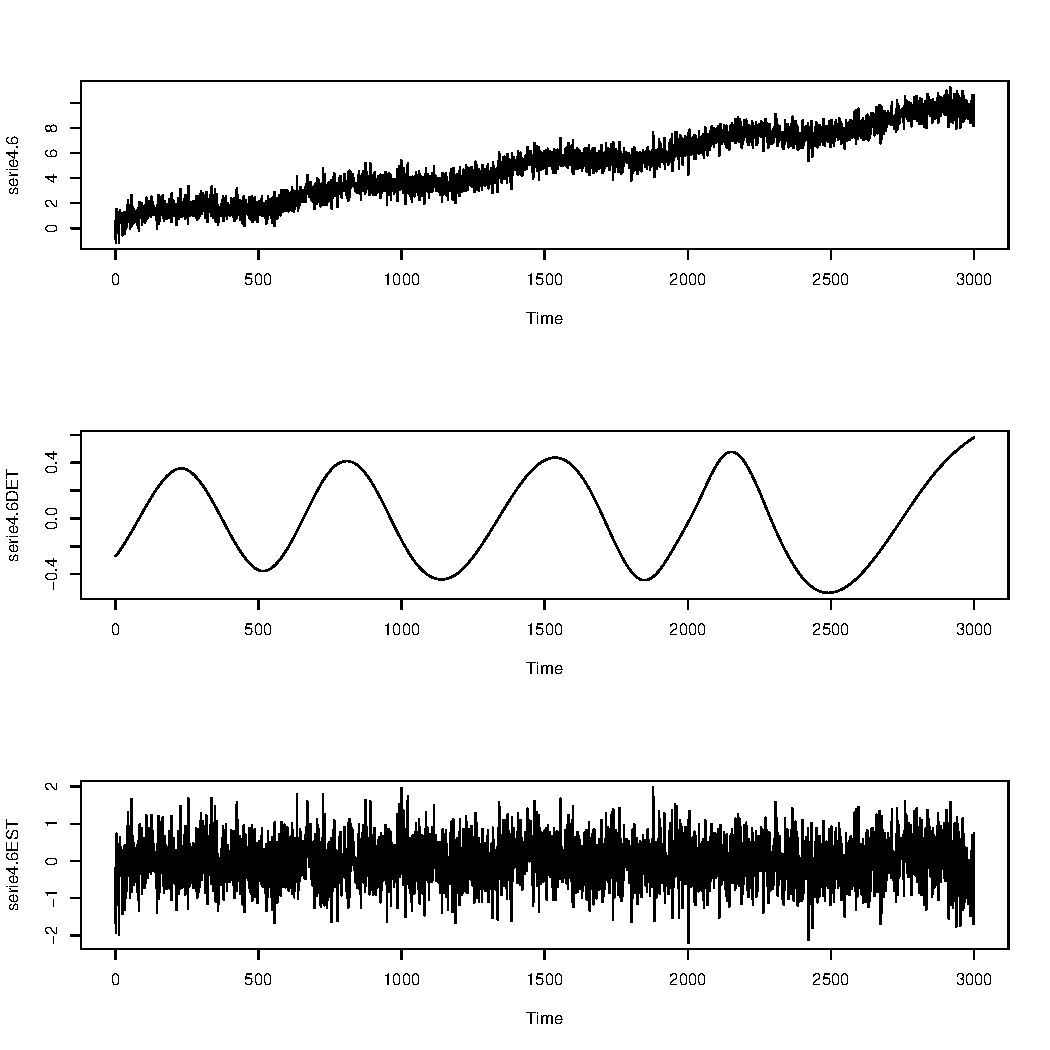
\includegraphics[scale=0.43]{serie4_6.pdf}
 \caption{Série 4.5 e Série 4.6}

\end{center}
\end{figure}

\graphicspath{{imagens/}}
\begin{figure}[H]
\begin{center}
  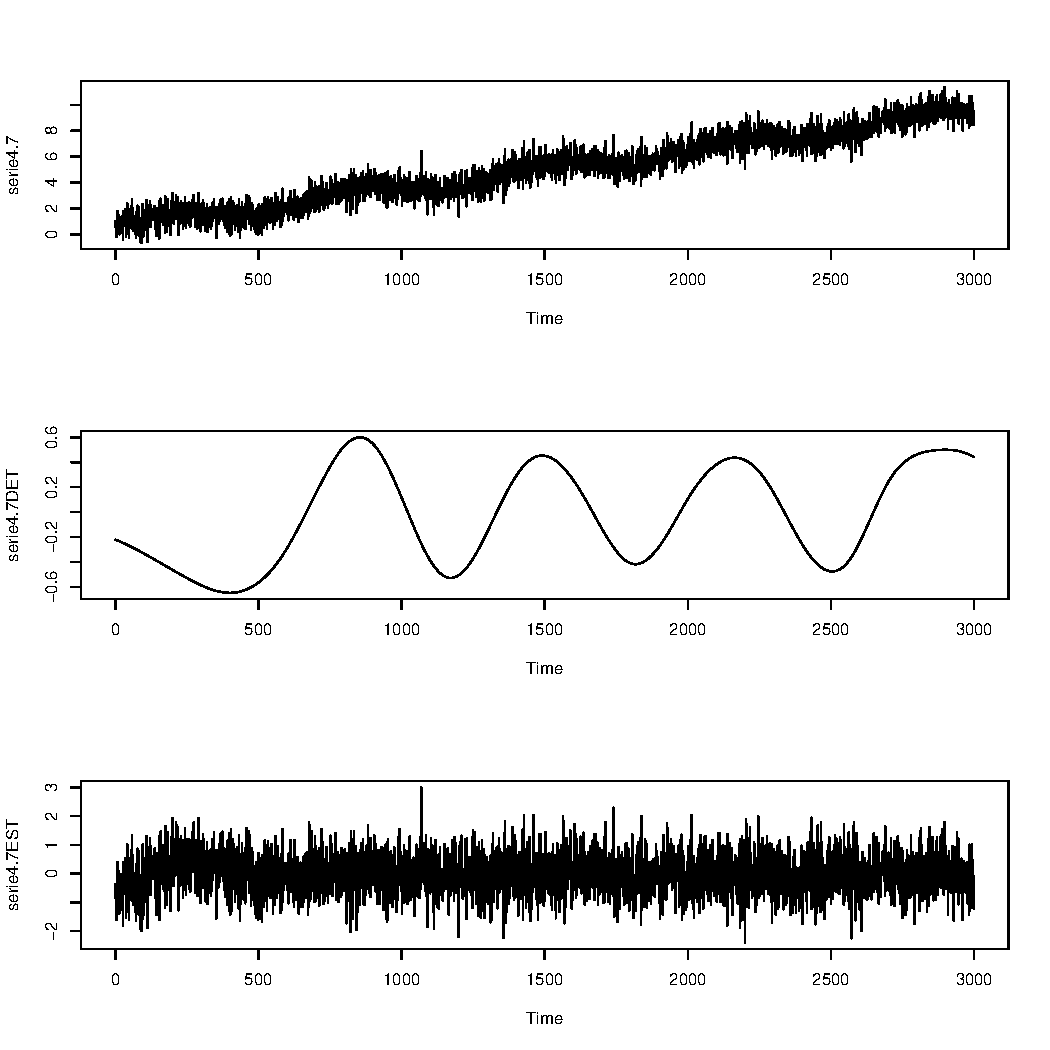
\includegraphics[scale=0.43]{serie4_7.pdf} \quad
  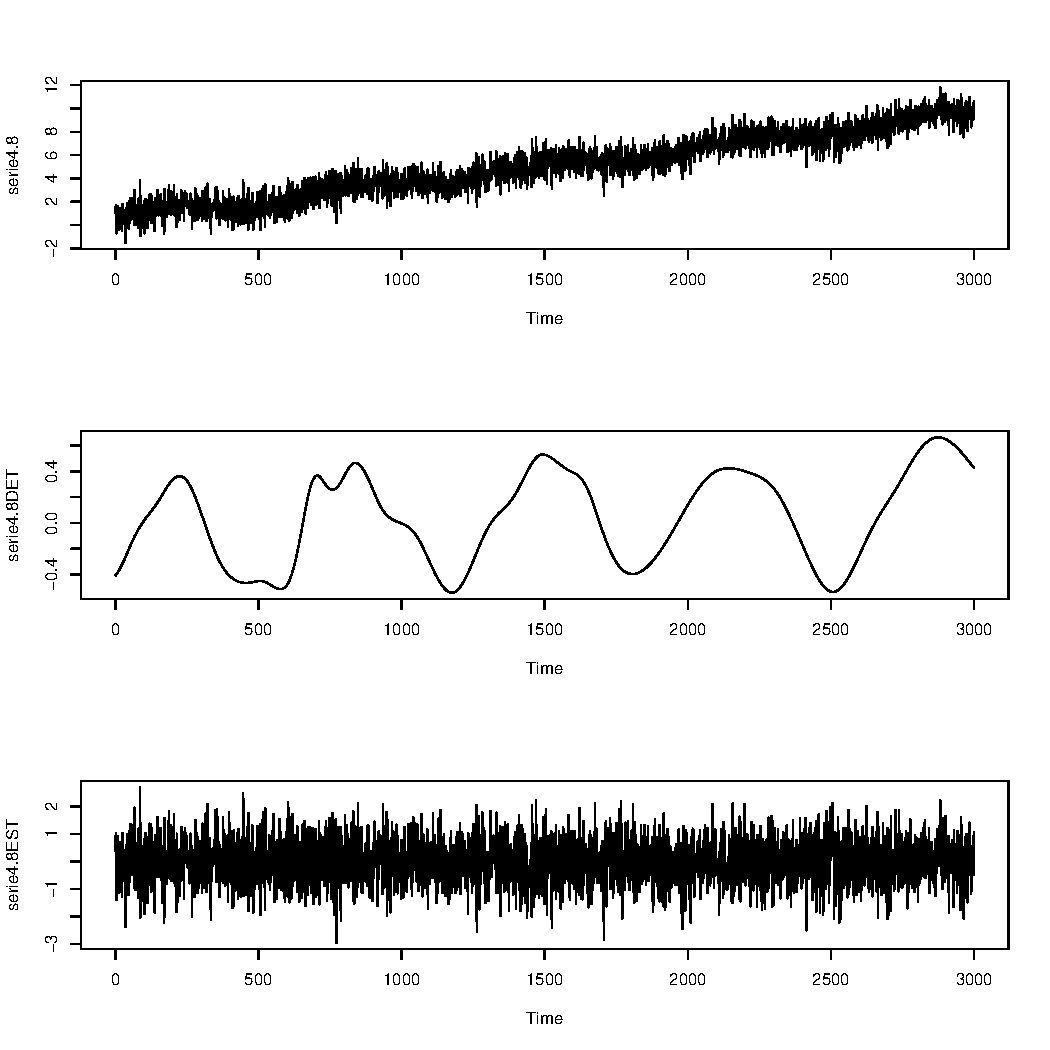
\includegraphics[scale=0.43]{serie4_8.pdf}
  \caption{Série 4.7 e Série 4.8}

\end{center}
\end{figure}

\graphicspath{{imagens/}}
\begin{figure}[H]
\begin{center}
  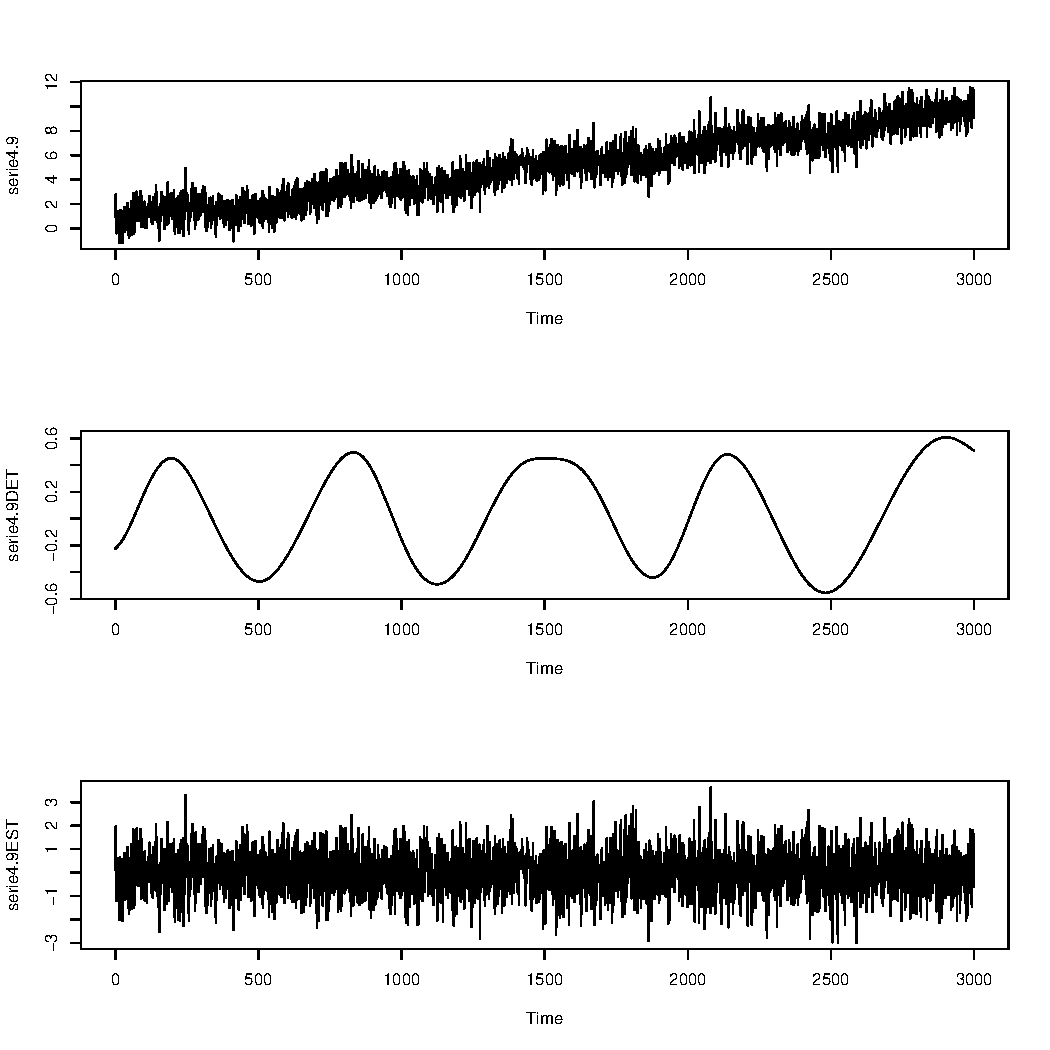
\includegraphics[scale=0.43]{serie4_9.pdf} \quad
  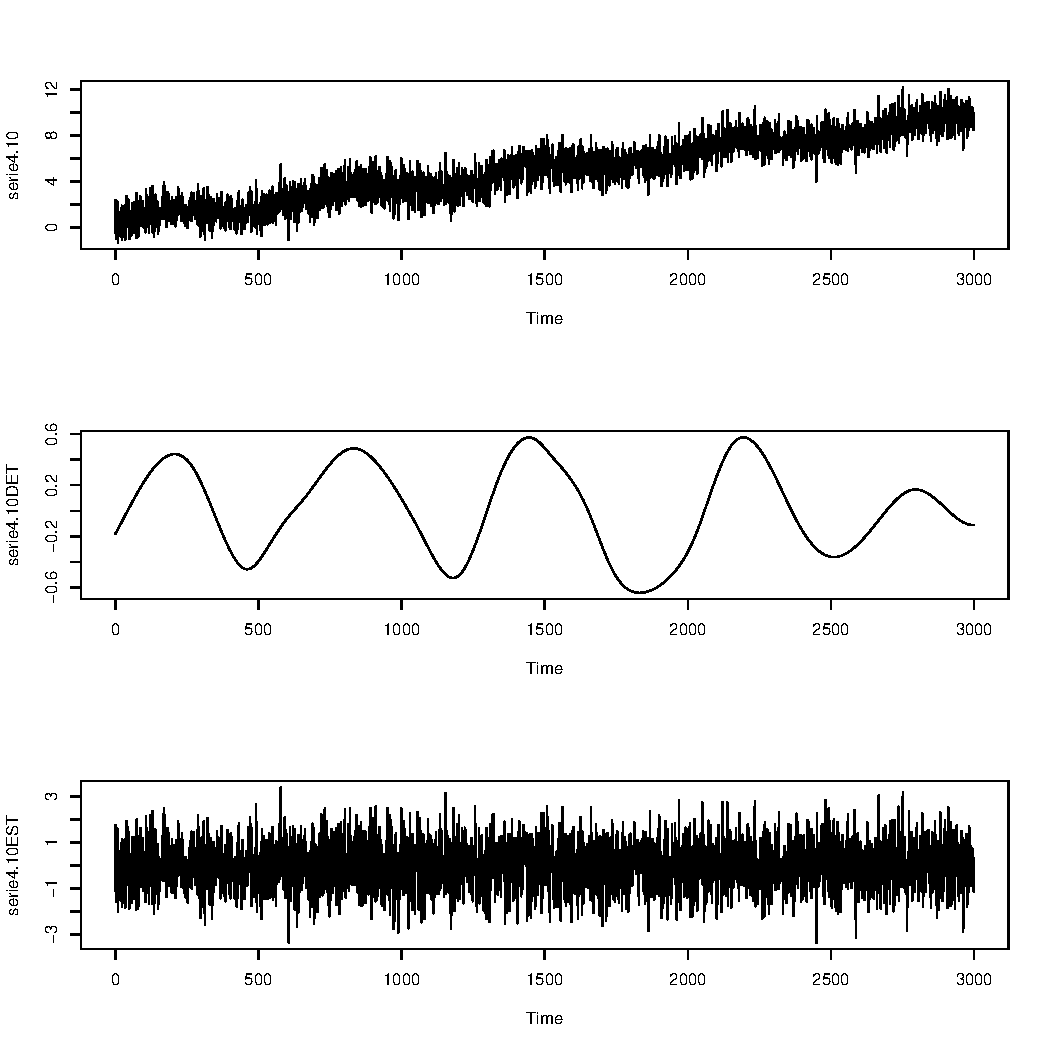
\includegraphics[scale=0.43]{serie4_10.pdf}
  \caption{Série 4.9 e Série 4.10}
\end{center}
\end{figure}
\section{Considerações Finais}
Foram apresentadas as séries temporais utilizadas neste trabalho experimental e suas respactivas decomposições.
% \include{apendice2}
% ...
% \include{apendiceM}

%% Fim do documento
\end{document}
%------------------------------------------------------------------------------------------%
